\documentclass[a4j,11pt]{jarticle}
\usepackage{fancyheadings}
\usepackage{here}
\usepackage[dvipdfmx]{graphicx}
\renewcommand{\thepage}{\small -- \arabic{page} --}
%\headrulewidth=0pt
\rhead{}
\lhead{}
\textheight 234mm
%
\usepackage{amsmath}	% required for `\cases' (yatex added)
\usepackage{bm}
\usepackage{ascmac}	% required for `\screen' (yatex added)
\usepackage{color}
\usepackage{listings,jvlisting}

\newcommand{\thisyear}{1}

\pagestyle{fancy}
\lhead{{\number\year}年度 メディア系演習I(画像情報処理)}

\title{{\number\year}年度 メディア系演習I\\ 画像情報処理 レポート}
\date{\number\year 年\number\month 月\number\day 日}

\author{グループA \\ 学籍番号32114006 \\ 飯田 諒}
%
%

\lstset{
   basicstyle={\ttfamily},
   identifierstyle={\small},
   commentstyle={\smallitshape},
   keywordstyle={\small\bfseries},
   ndkeywordstyle={\small},
   stringstyle={\small\ttfamily},
   frame={tb},
   breaklines=true,
   columns=[l]{fullflexible},
   numbers=left,
   xrightmargin=0zw,
   xleftmargin=3zw,
   numberstyle={\scriptsize},
   stepnumber=1,
   numbersep=1zw,
   lineskip=-0.5ex
}

\begin{document}
%
\maketitle
\clearpage
%
%
\section{はじめに}
%
%
今回は画像情報処理の方法について学んだことを記す。
%
%
\section{実験内容}
%
%
\subsection{演習1:アフィン変換による画像の回転}

\subsubsection{ディレクトリ01に移動せよ}
\$cd IP-CSE/01を実行することで、移動できた。
\subsubsection{アフィン変換のプログラムを実装せよ}
%\begin{lstlisting}[caption = アフィン変換,label=fuga]
%void affine_transformation(Mat& input, Mat& output,double sx, double sy, double theta, int tx, int ty) {
%  // アフィン変換を行う
%  for(int x=0;x<input.size().width;x++){
%    for(int y=0;y<input.size().height;y++){
%      for(int c=0;c<input.channels();c++){
%        setPixel(output,x,y,c,0);
%        int dx = ((x-tx)$\times$cos(theta/180$\times$M_PI)+(y-ty)$\times$sin(theta/180$\times$M_PI))/sx;
%        int dy = (-(x-tx)$\times$sin(theta/180$\times$M_PI)+(y-ty)$\times$cos(theta/180$\times$M_PI))/sy;
%        if(dx<0||input.size().width<=dx||dy<0||input.size().height<=dy){continue;}
%        setPixel(output,x,y,c,getPixel(input,dx,dy,c));

%      }
%    }
%  }
%}
%\end{lstlisting}
\subsubsection{回転角度を60度、135度に設定し、出力を得よ。その際、画面の橋が着れないようにすること。}
\clearpage
\begin{figure}[tb]

 \center
 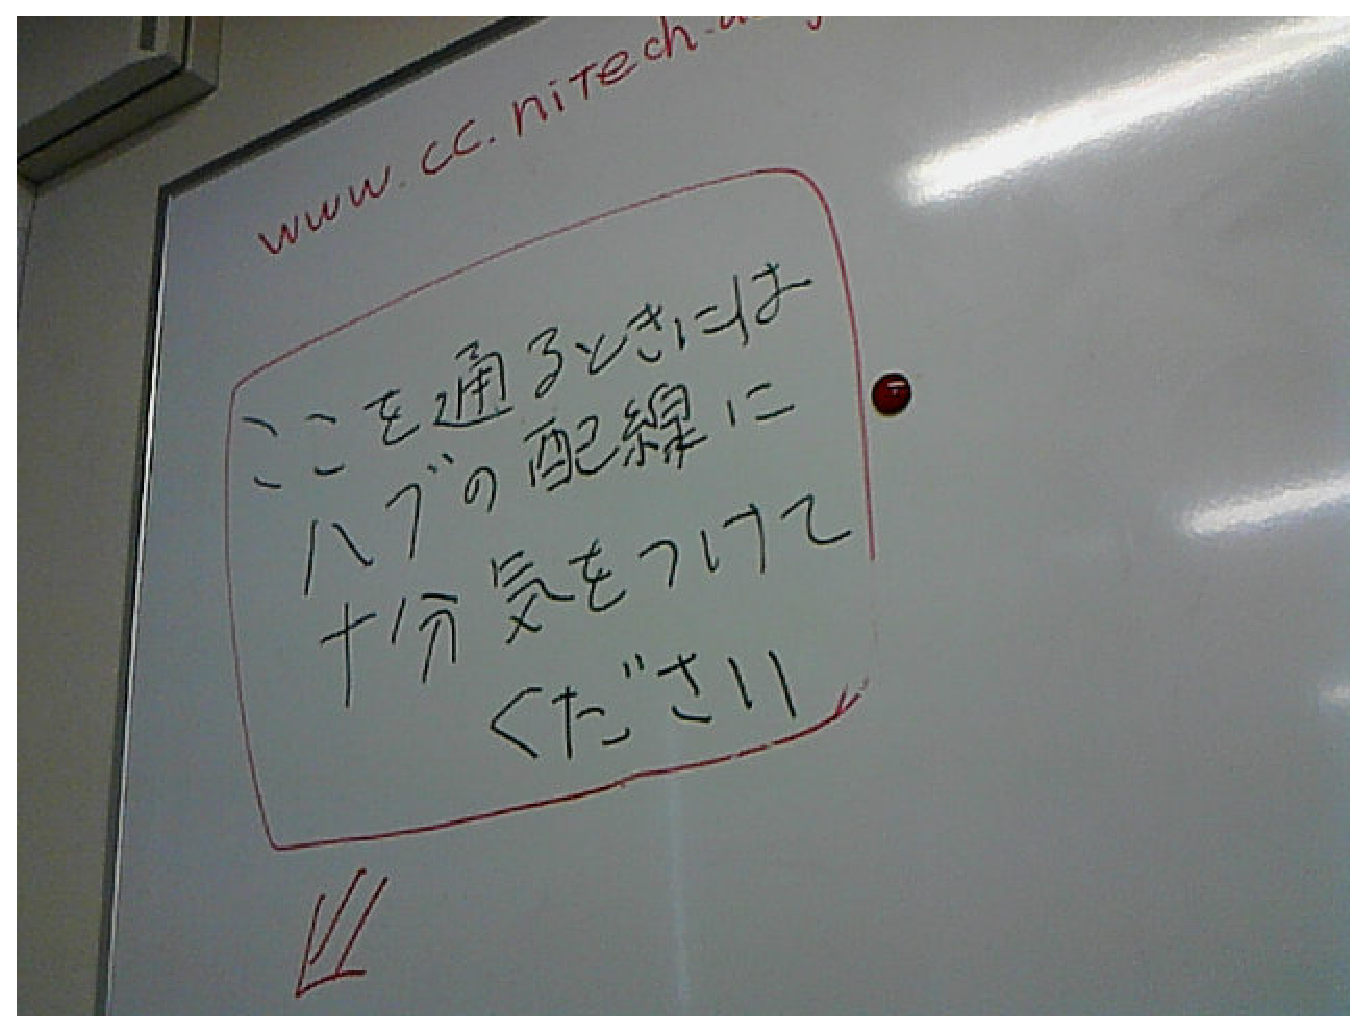
\includegraphics[width=0.8\hsize]{./eps/input.eps}
 %% 横幅 x 0.8 のサイズで図を掲載
   %% 最近はPDFファイルの使用が推奨されている(容量についても減少させやすい)
 \\図1:元画像
 \label{fig:affine1}

 \begin{minipage}{0.49\hsize} % 横幅 x 0.49 のサイズで分割
   \center
   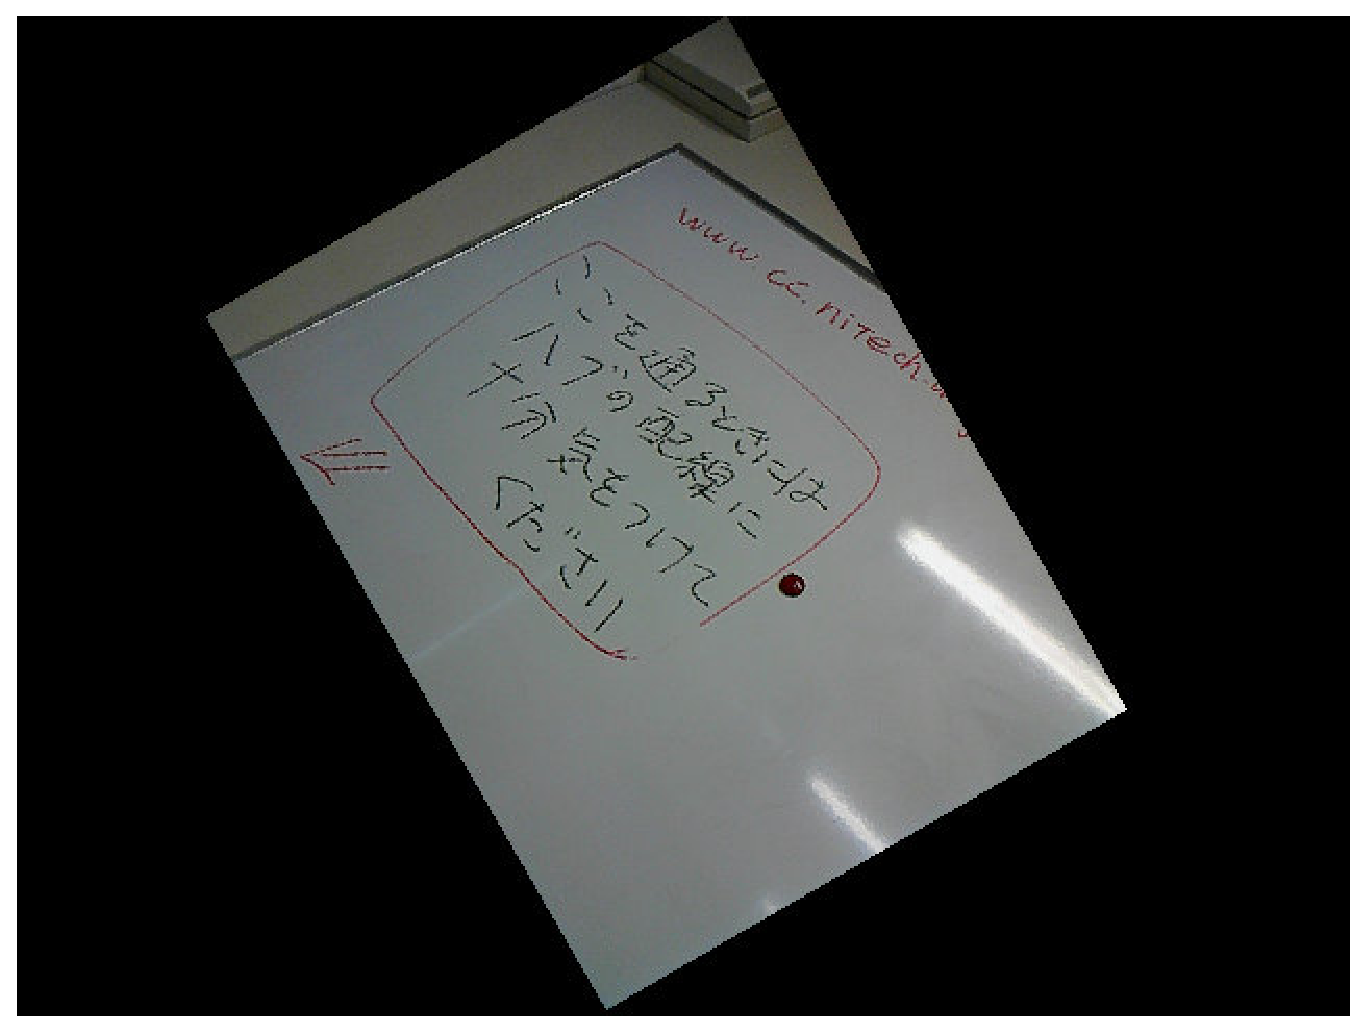
\includegraphics[width=\hsize]{./eps/affine-60.eps}
   %% 分割されたサイズぴったりに図を掲載(width=\hsize)
   図2:アフィン変換による60度回転
 \end{minipage}
 \begin{minipage}{0.49\hsize} % 横幅 x 0.49 のサイズで分割
   \center
   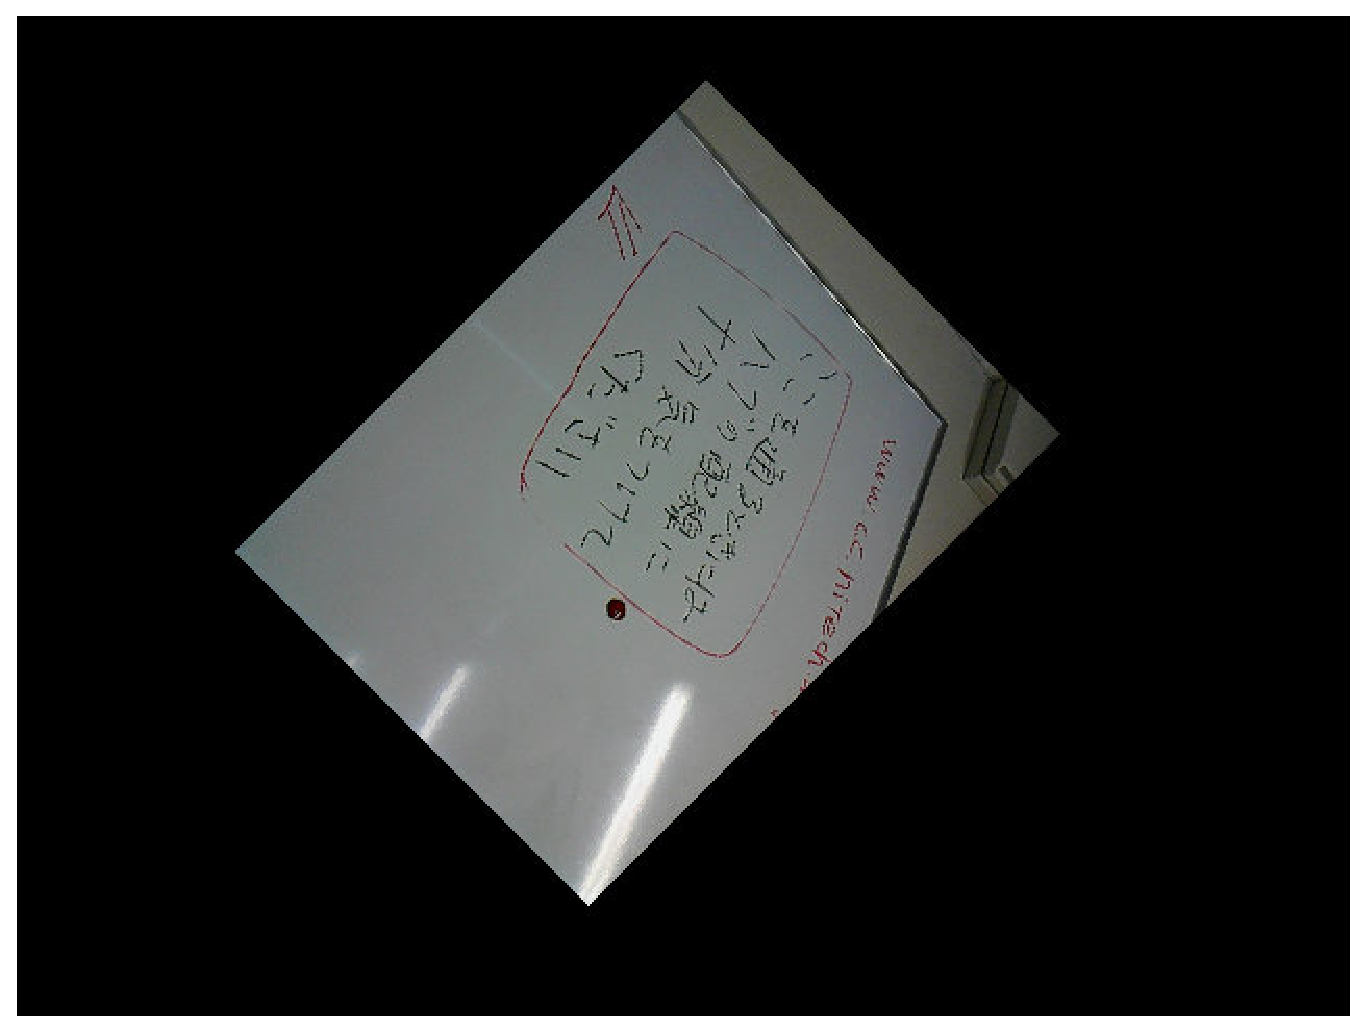
\includegraphics[width=\hsize]{./eps/affine-135.eps}

   %% 分割されたサイズぴったりに図を掲載(width=\hsize)
   図3:アフィン変換による135度回転
 \end{minipage}
% \caption{minipageの使用例}
 \label{fig:affine2}
\end{figure}
\subsubsection{知見と考察}
今回私はアフィン変換の逆変換の実装を行った。
逆変換による実装を用いることによって、出力側から入力側の画像を検索するので、
出力画像中の抜けが発生しないことが保証されるのである。
実際に上記の図から読み取れる通り、アフィン変換後の画像は周りの黒い画素以外のところでは抜けが発生していない。
%
%

%
\subsection{演習2:平滑化フィルタによる処理}

\subsubsection{移動平均フィルタのプログラムを実装せよ。}
\subsubsection{移動平均フィルタのオペレータを3$\times$3、5$\times$5と変化させ、出力結果を比較せよ。}
\clearpage
\clearpage
\begin{figure}[tb]

% \center
% 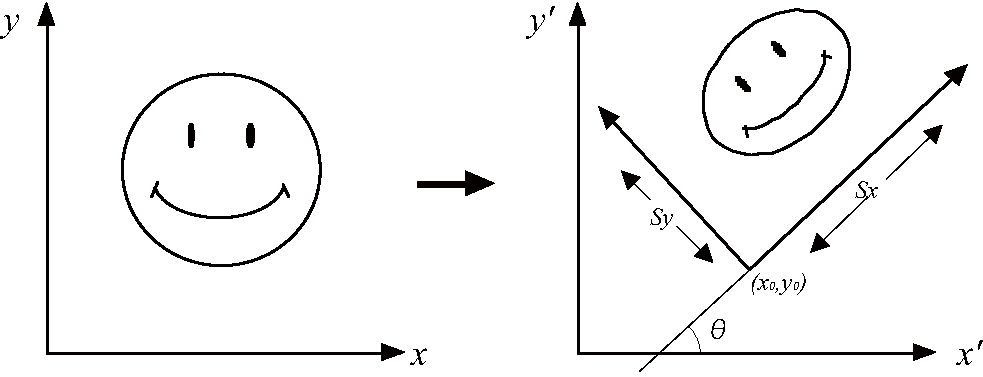
\includegraphics[width=0.8\hsize]{./fig/affine.pdf}
 %% 横幅 x 0.8 のサイズで図を掲載
   %% 最近はPDFファイルの使用が推奨されている(容量についても減少させやすい)
% \caption{アフィン変換の例}
% \label{fig:affine1}

 \begin{minipage}{0.49\hsize} % 横幅 x 0.49 のサイズで分割
   \center
   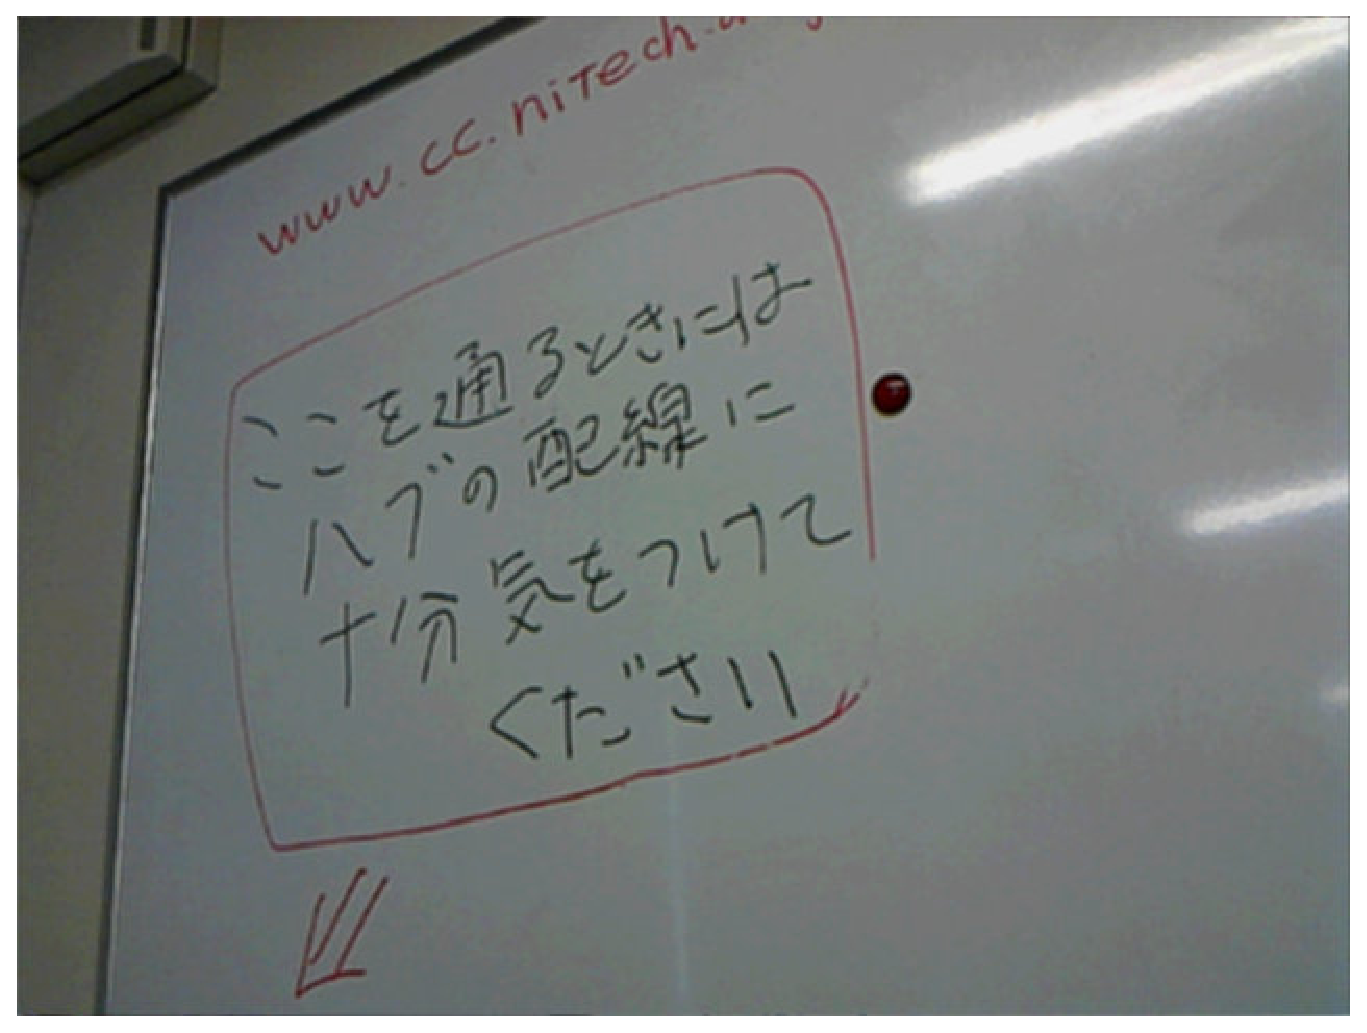
\includegraphics[width=\hsize]{./eps/smooth-movingAverage-dim3.eps}
   %% 分割されたサイズぴったりに図を掲載(width=\hsize)
   図4:3$\times$3移動平均フィルタ
 \end{minipage}
 \begin{minipage}{0.49\hsize} % 横幅 x 0.49 のサイズで分割
   \center
   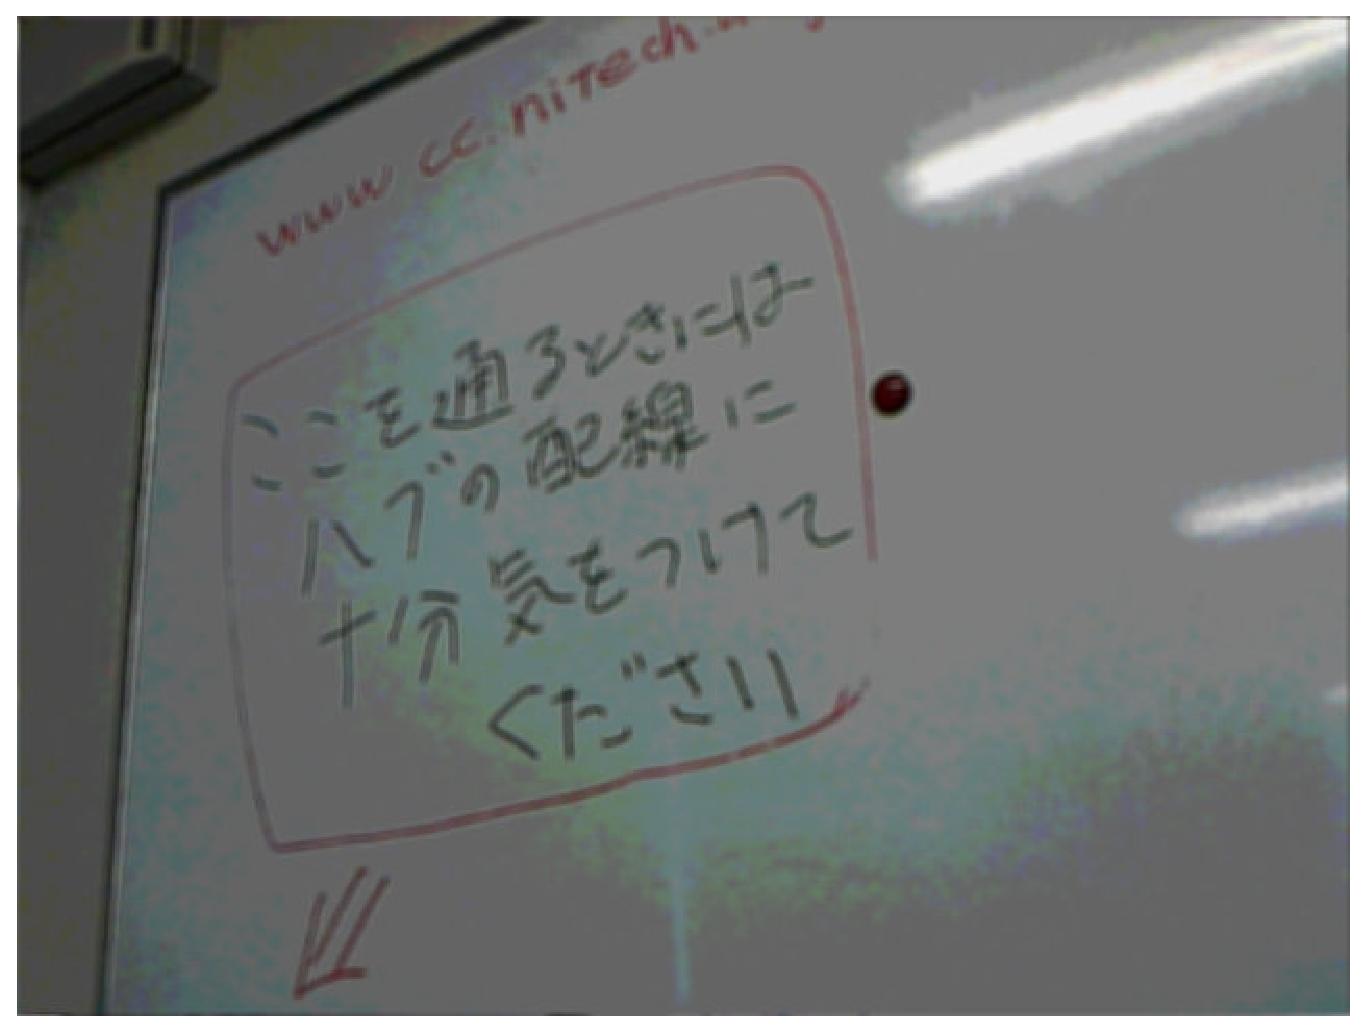
\includegraphics[width=\hsize]{./eps/smooth-movingAverage-dim5.eps}

   %% 分割されたサイズぴったりに図を掲載(width=\hsize)
   図5:5$\times$5移動平均フィルタ
 \end{minipage}
% \caption{minipageの使用例}
 \label{fig:affine2}
\end{figure}
\subsubsection{入力画像にノイズを混入させ、実験結果よりノイズ除去について考察せよ。}
\clearpage
\begin{figure}[tb]

 \center
 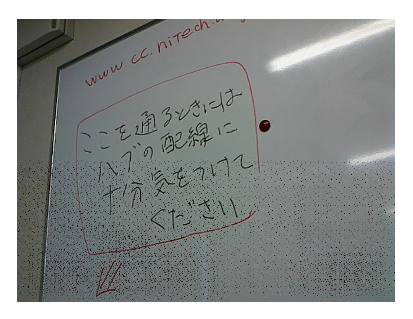
\includegraphics[width=0.8\hsize]{./eps/noiz.eps}
 %% 横幅 x 0.8 のサイズで図を掲載
   %% 最近はPDFファイルの使用が推奨されている(容量についても減少させやすい)
 \\図6:ノイズのある画像
 \label{fig:affine1}

 \begin{minipage}{0.49\hsize} % 横幅 x 0.49 のサイズで分割
   \center
   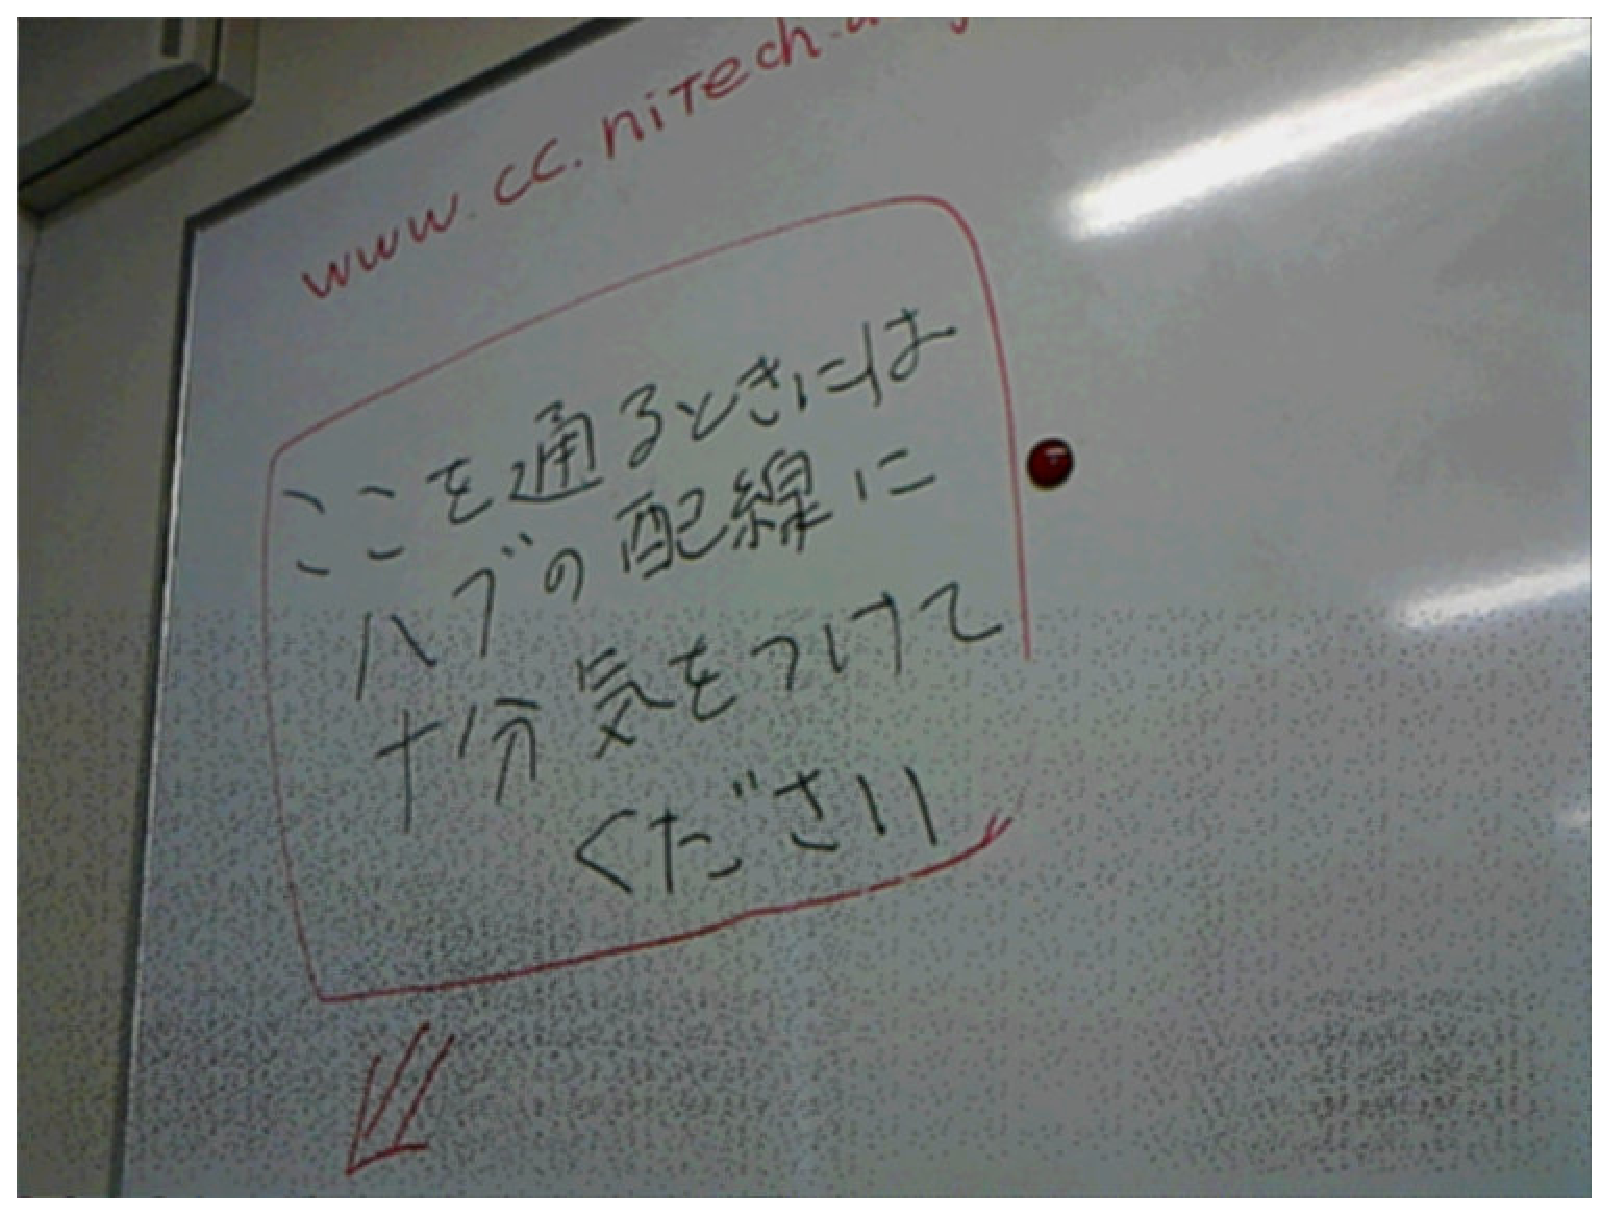
\includegraphics[width=\hsize]{./eps/smooth-noiz-movingAverage-dim3.eps}
   %% 分割されたサイズぴったりに図を掲載(width=\hsize)
   図7:ノイズに対する3$\times$3移動平均フィルタ
 \end{minipage}
 \begin{minipage}{0.49\hsize} % 横幅 x 0.49 のサイズで分割
   \center
   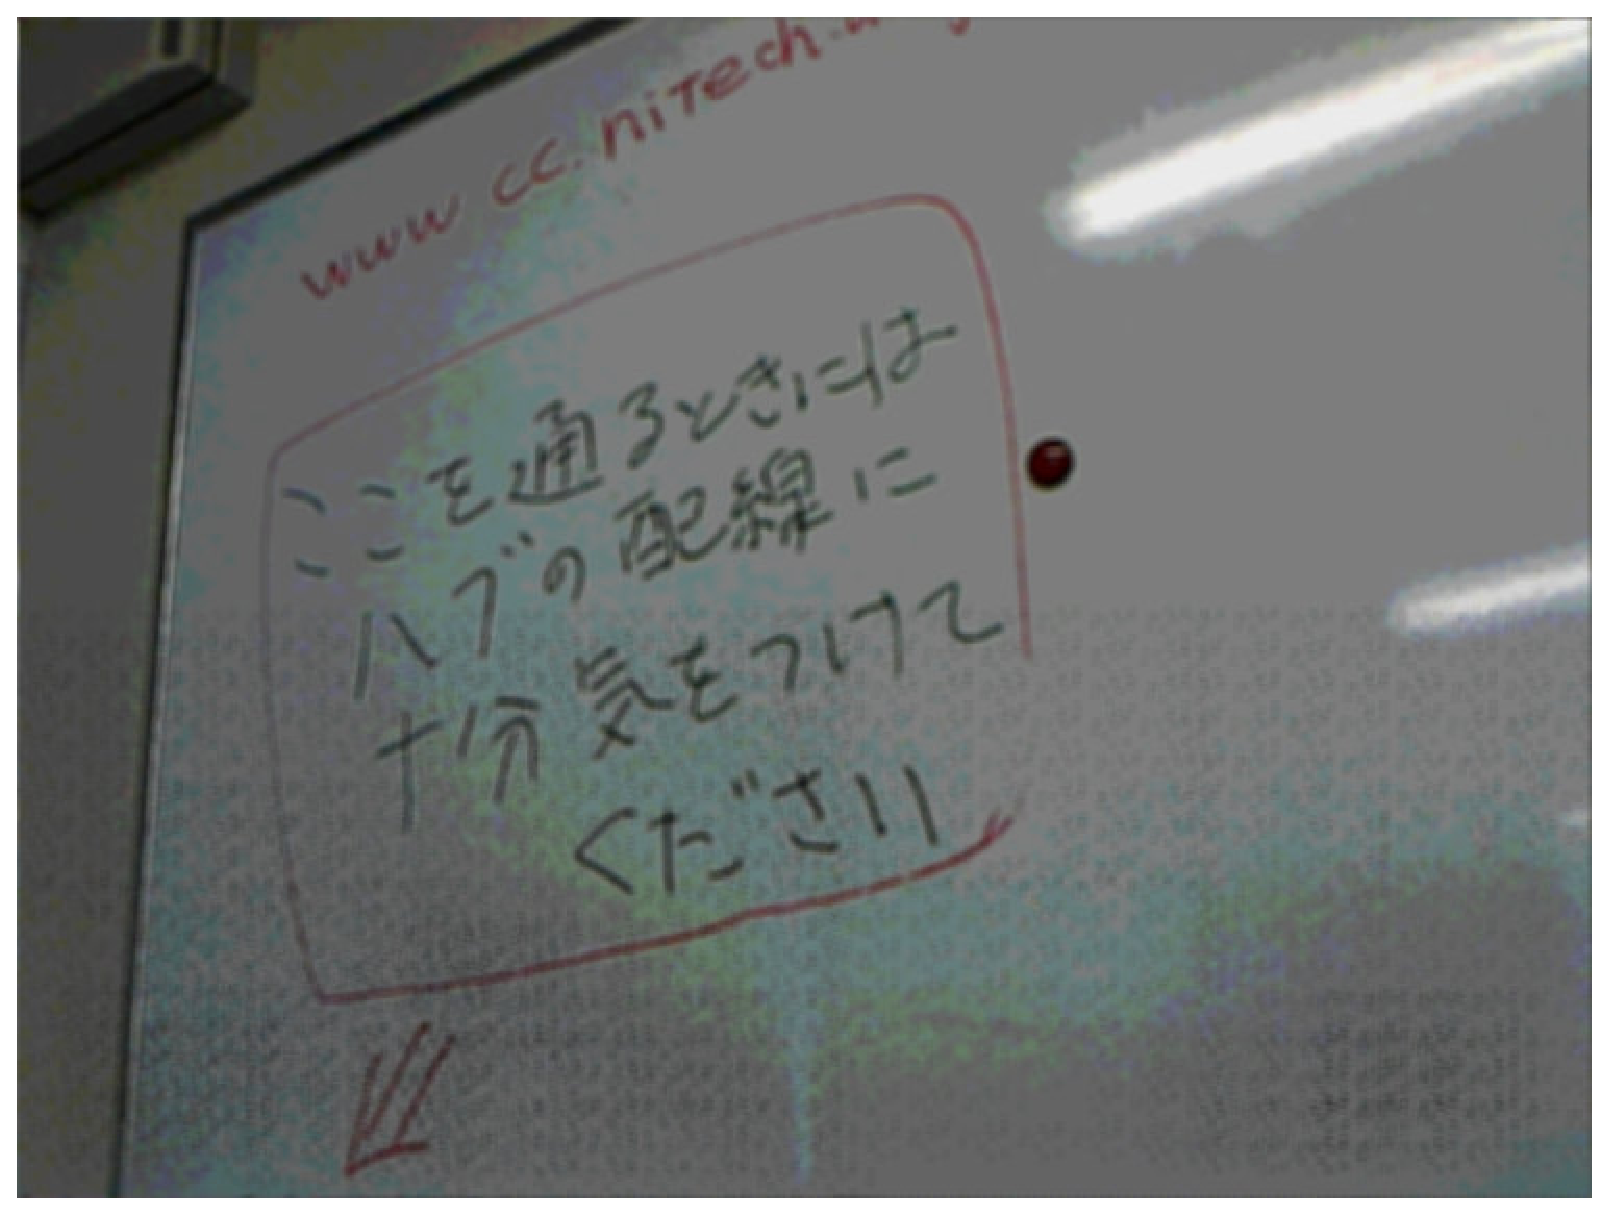
\includegraphics[width=\hsize]{./eps/smooth-noiz-movingAverage-dim5.eps}

   %% 分割されたサイズぴったりに図を掲載(width=\hsize)
   図8:ノイズに対する5$\times$5移動平均フィルタ
 \end{minipage}
% \caption{minipageの使用例}
 \label{fig:affine2}
\end{figure}
考察は次セクションの知見と考察で示す。
\subsubsection{知見と考察}
移動平均フィルタは以下の行列を用いる。\\
3$\times$3移動平均フィルタ
$$
\begin{pmatrix}
  \frac1 9 & \frac1 9 & \frac1 9 \\
  \frac1 9 & \frac1 9 & \frac1 9 \\
  \frac1 9 & \frac1 9 & \frac1 9  

\end{pmatrix}
$$

5$\times$5移動平均フィルタ
$$
\begin{pmatrix}
  \frac1 {25} & \frac1 {25} & \frac1 {25} & \frac1 {25} & \frac1 {25}\\
  \frac1 {25} & \frac1 {25} & \frac1 {25} & \frac1 {25} & \frac1 {25}\\
  \frac1 {25} & \frac1 {25} & \frac1 {25} & \frac1 {25} & \frac1 {25}\\
  \frac1 {25} & \frac1 {25} & \frac1 {25} & \frac1 {25} & \frac1 {25}\\
  \frac1 {25} & \frac1 {25} & \frac1 {25} & \frac1 {25} & \frac1 {25}
\end{pmatrix}
$$
ある画素が、周辺の画素の色と違った色をしているとき、そのある画素は移動平均フィルタによって周囲の色によって平均化されることにより、
その違った色が薄れ、周囲の色に近づく。これにより、ノイズが除去される。\\
二つ目の演習において、元画像に比べてフィルタを通した後では、ホワイトボードと文字の境界線が少しぼやけていて、文字が太くなっている。
また、全体的にピントがあっていないように見える。また、ホワイトボードに反射している蛍光灯は、白色がホワイトボードに絵の具がにじんだように侵食している。
よって、移動平均フィルタを用いると、画像全体がぼやけてしまうことが読み取れる。また、3$\times$3と5$\times$5のフィルタを使ったときに違いについて、5$\times$5の画像の方がさらにぼやけている。
これは平滑化の範囲が広いことによることであると考える。また、
ホワイトボードの画素から影の影響によって黄色や青の画素が出現している。これは、今回の実装において赤青黄の値それぞれ独立に操作したためであると考える。
よって、次数の高い移動平均フィルタを用いると、さらにぼやけたり、ありもしない色が出現してしまったりなど弊害が出てしまう。\\
三つ目の演習において、ノイズのある画像に移動平均フィルタを通すと、元画像に比べてノイズが薄れている。また、3$\times$3より次数の多い5*5の方が薄れている。これは、画像がぼやける代わりにノイズもぼやけることによって
目立たなくなっていることが考えられる。以上より、移動平均フィルタを用いると、欠点として、画像全体がぼやけてしまったり、次数が高いフィルタを用いるとありもしない色が出現してしまうが、
利点として、ノイズが目立たなくなることが挙げられるので、適切な次数を選んで用いるとノイズのある画像に対して有用性があると考えた。
%
%
\subsection{演習3:エッジ検出フィルタによる処理}

\subsubsection{Sobelフィルタのプログラムを実装せよ。}
\subsubsection{水平、垂直、斜め方向のエッジに関して出力画像を用いて考察せよ。}
フィルタによる効果が分かりやすい境界がはっきりしている画像を用いた。
\clearpage
\begin{figure}[tb]

 \center
 
\includegraphics[width=0.7\hsize]{./eps/squares.eps}
 %% 横幅 x 0.8 のサイズで図を掲載
   %% 最近はPDFファイルの使用が推奨されている(容量についても減少させやすい)
\\ 図9:元画像\\
 \label{fig:affine1}
 \begin{minipage}{0.49\hsize} % 横幅 x 0.49 のサイズで分割
   \center
   
\includegraphics[width=0.7\hsize]{./eps/edge-sobelx.eps}
   %% 分割されたサイズぴったりに図を掲載(width=\hsize)
   \\図10:Sobelフィルタによる水平方向の検出
 \end{minipage}
 \clearpage
 \begin{minipage}{0.49\hsize} % 横幅 x 0.49 のサイズで分割
   \center
   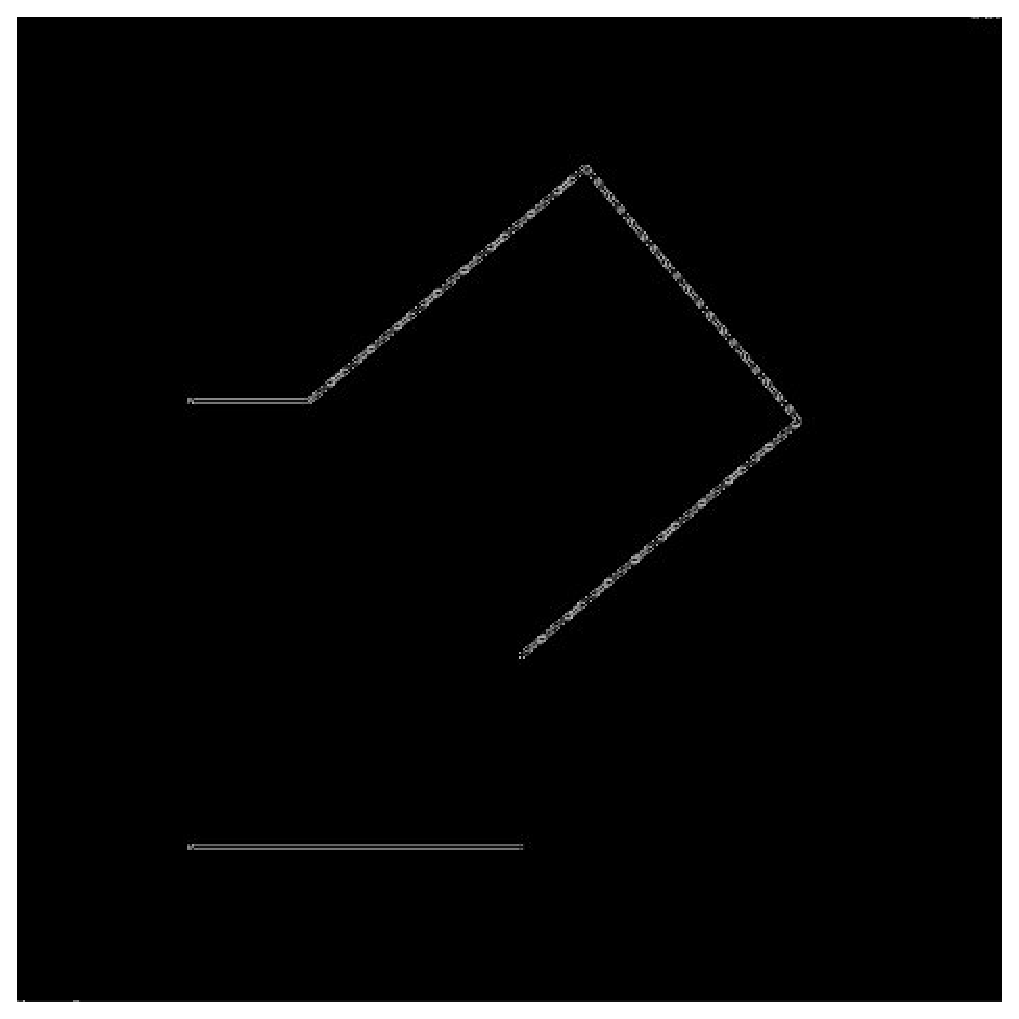
\includegraphics[width=0.7\hsize]{./eps/edge-sobely.eps}

   %% 分割されたサイズぴったりに図を掲載(width=\hsize)
   図11:Sobelフィルタによる垂直方向の検出
 \end{minipage}
%  \caption{Sobelフィルタの適応}
 \label{fig:affine2}
\end{figure}
考察は次セクションの知見と考察で示す。
\subsubsection{知見と考察}
Sobelフィルタは以下の二つの行列を用いる。\\

水平方向フィルタ
$$
\begin{pmatrix}
  -1 & 0 & 1 \\
  -2 & 0 & 2 \\
  -1 & 0 & 1 
\end{pmatrix}
$$
垂直方向フィルタ
$$
\begin{pmatrix}
  -1 & -2 & -1 \\
   0 &  0 & 0 \\
   1 &  2 & 1 
\end{pmatrix}
$$
上記のフィルタを用いるとそれぞれ水平方向、垂直方向に敏感なエッジが出力された。
しかし画像中央の下辺りの左から黒から白へ変化している部分に関してはどちらのフィルタに関しても検出されなかった。
\(フィルタA、フィルタBをそれぞれ回転させても結果は変わらなかった。\)
よって、右から左に黒から白、つまり暗い画素から明るい画素に変わっている境界に関しては検出されないことがわかる。
斜め方向についてはどちらのフィルタを用いても検出することができた。実用的にSobelフィルタを用いるときには水平方向と垂直方向の出力画像のノルムをとった
ものを用いれば実用性があると考えた。

\subsection{応用課題1:平滑化フィルタによる処理}

\subsubsection{移動平均フィルタ以外の平滑かフィルタについて調査・実装せよ。}
図6のノイズのある画像にガウシアンフィルタを用いて調査・実装した。
\clearpage
\begin{figure}[tb]


  \begin{minipage}{0.49\hsize} % 横幅 x 0.49 のサイズで分割
   \center
   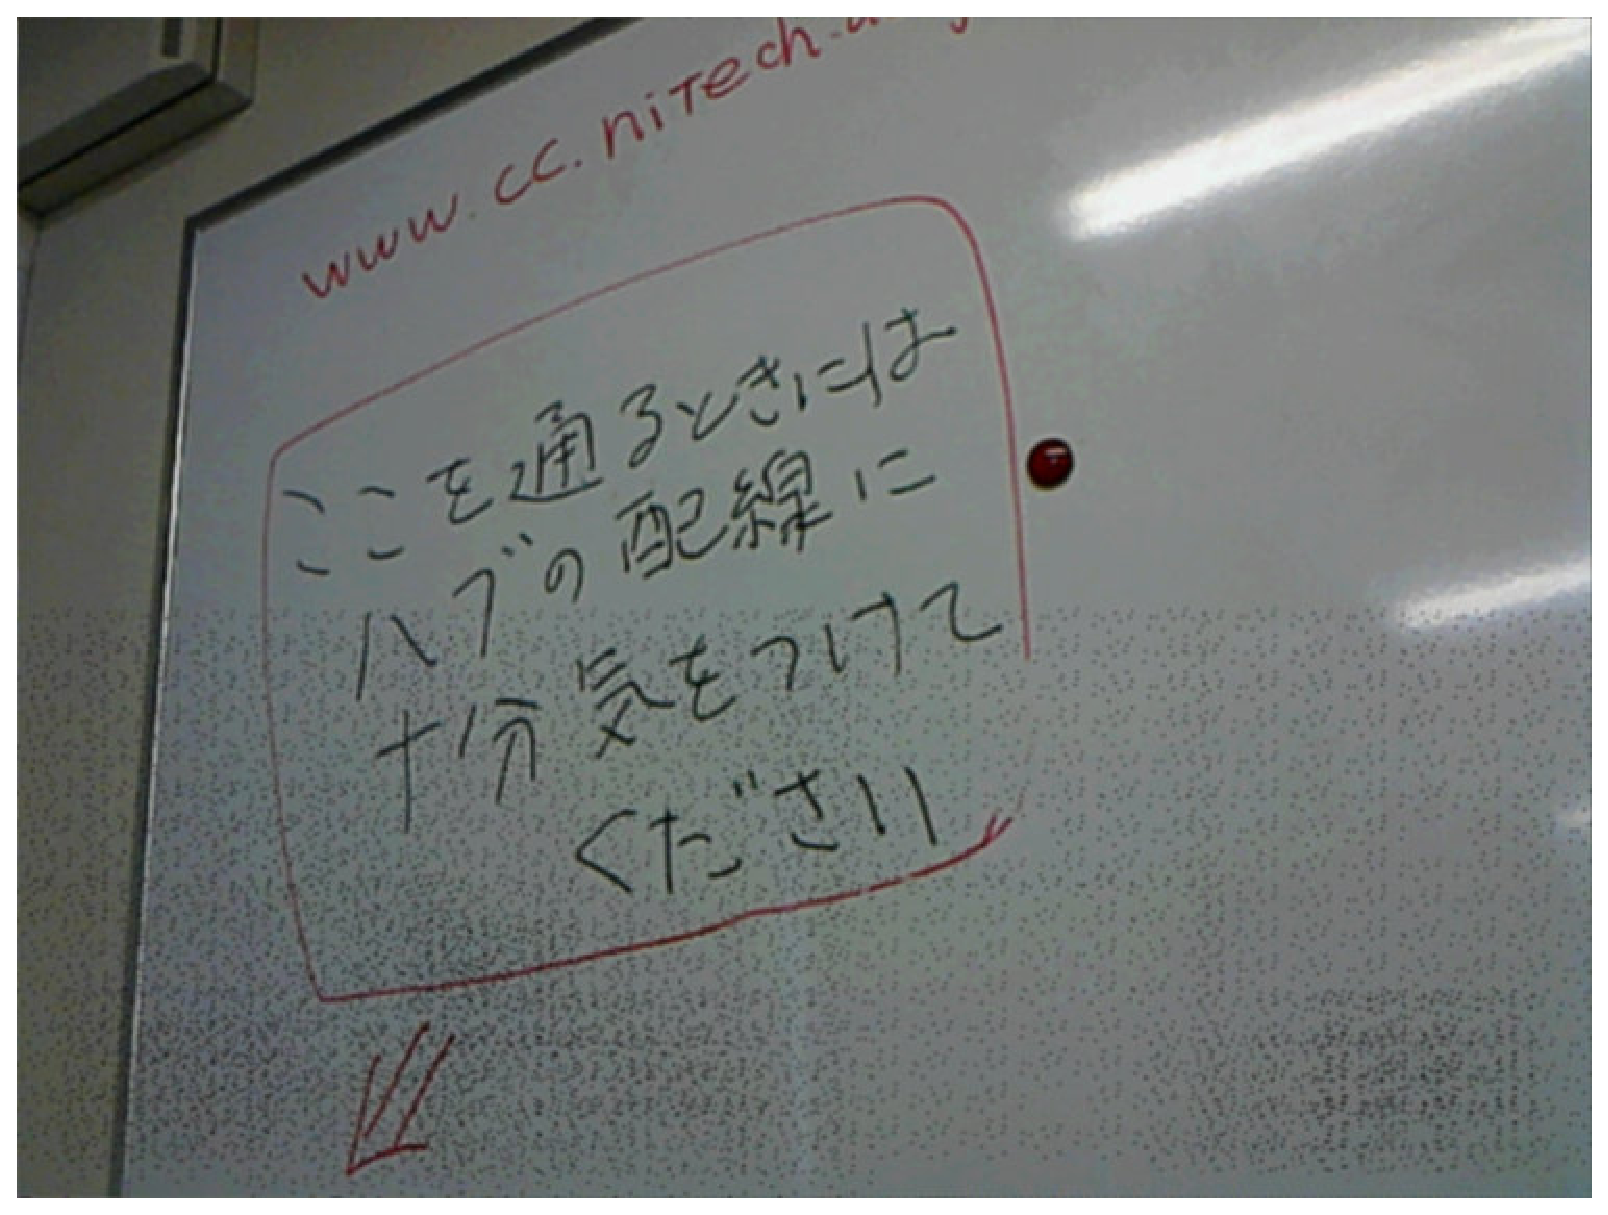
\includegraphics[width=\hsize]{./eps/smooth-noiz-gaussian-dim3.eps}
   %% 分割されたサイズぴったりに図を掲載(width=\hsize)
   図12:3$\times$3ガウシアンフィルタ
 \end{minipage}
 \begin{minipage}{0.49\hsize} % 横幅 x 0.49 のサイズで分割
   \center
   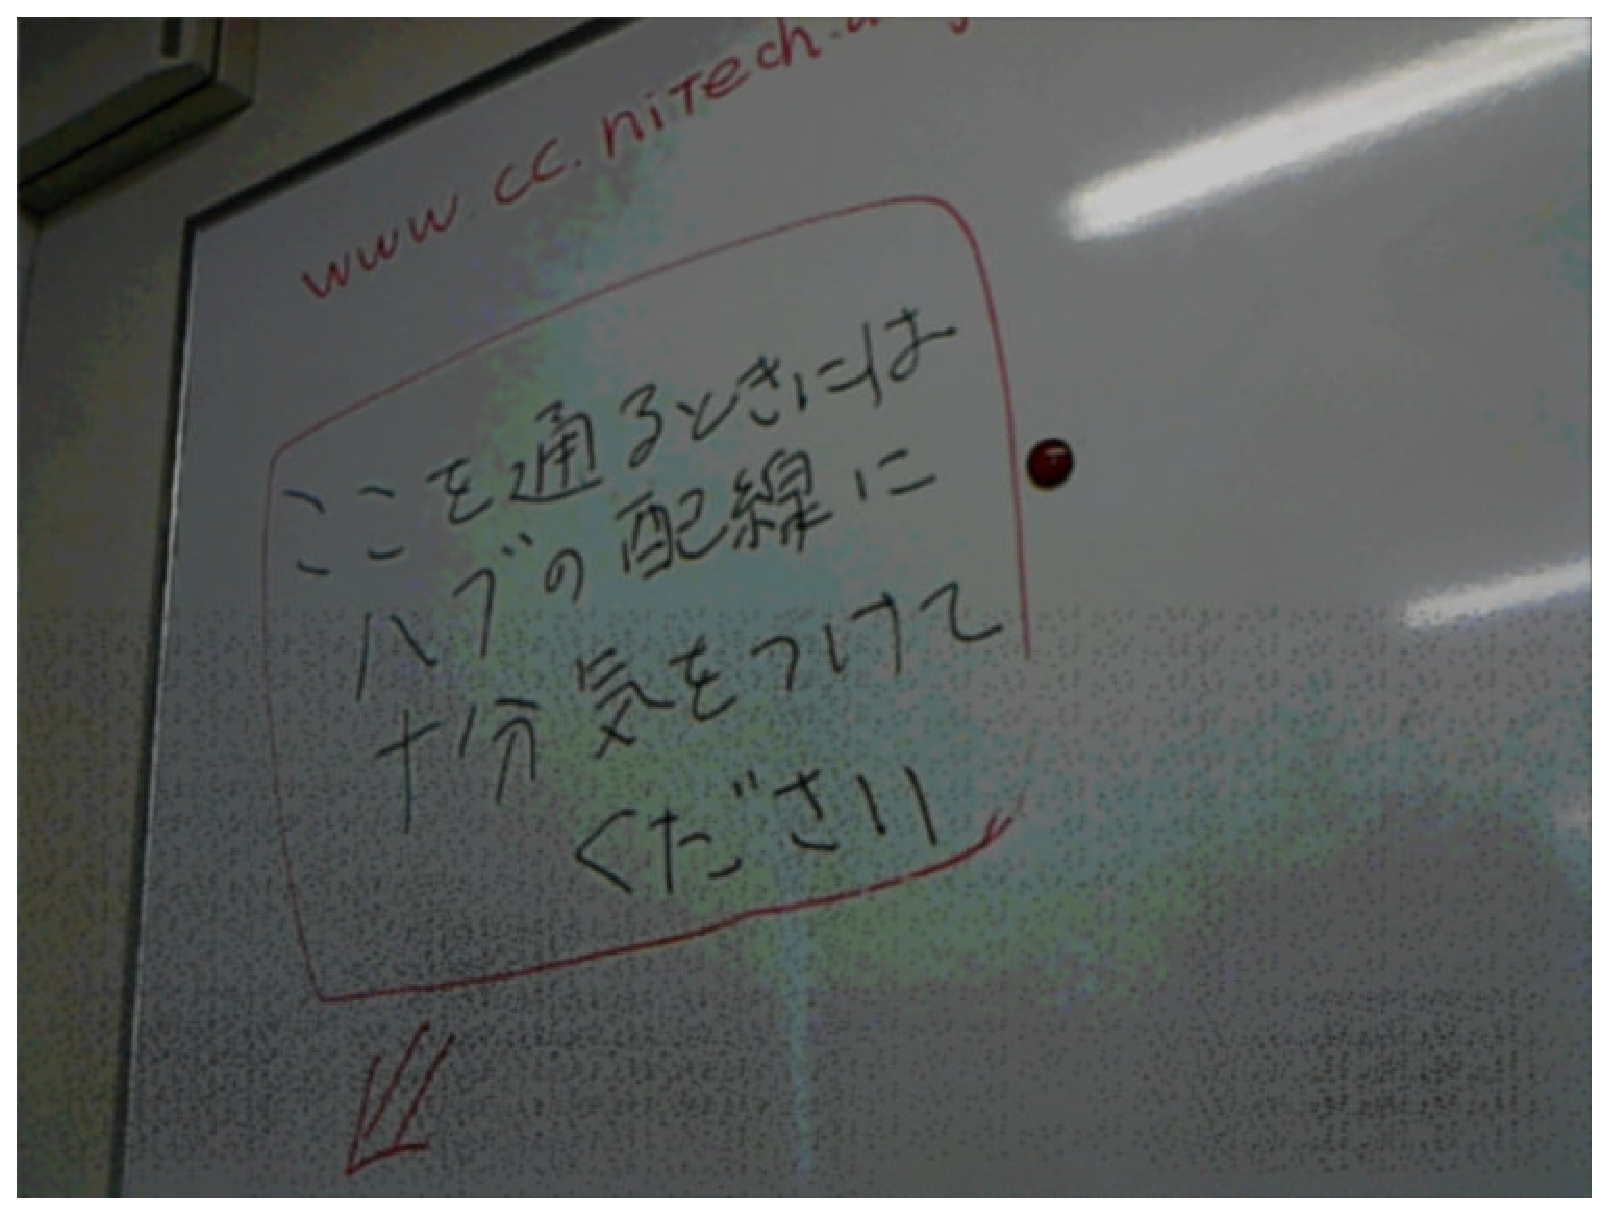
\includegraphics[width=\hsize]{./eps/smooth-noiz-gaussian-dim5.eps}

   %% 分割されたサイズぴったりに図を掲載(width=\hsize)
   図13:5$\times$5ガウシアンフィルタ
 \end{minipage}
%  \caption{minipageの使用例}
 \label{fig:affine2}
\end{figure}
\subsubsection{そのフィルタの特性等について考察せよ}
ガウシアンフィルタは以下の通りである。\\
3$\times$3ガウシアンフィルタ
$$
\begin{pmatrix}
  \frac1 {16} & \frac2 {16} & \frac1 {16} \\
  \frac2 {16} & \frac4 {16} & \frac2 {16} \\
  \frac1 {16} & \frac2 {16} & \frac1 {16}  

\end{pmatrix}
$$

5$\times$5ガウシアンフィルタ
$$
\begin{pmatrix}
  \frac1 {256} & \frac4 {256} & \frac6 {256} & \frac4 {256} & \frac1 {256}\\
  \frac4 {256} & \frac6 {256} & \frac{24} {256} & \frac6 {256} & \frac4 {256}\\
  \frac6 {256} & \frac{24} {256} & \frac{36} {256} & \frac{24} {256} & \frac6 {256}\\
  \frac4 {256} & \frac6 {256} & \frac{24} {256} & \frac6 {256} & \frac4 {256}\\
  \frac1 {256} & \frac4 {256} & \frac6 {256} & \frac4 {256} & \frac1 {256}
\end{pmatrix}
$$
移動平均フィルタを通したときと比べると、ノイズの軽減が少ない。これは二次元のガウス関数の形において、
原点において盛り上がっていることが原因で、周りの画素に影響される割合が、移動平均フィルタに比べて少ないことが考察できる。
よって、ノイズの軽減を少し押さえたいが、画像全体はこれ以上ぼかしたくなかったときに有用性があると考える。
またこれについて、例として、フィルタにできる最小の次数は奇数という制約の元3であるので、3$\times$3移動平均フィルタを通したときに
画像全体のぼけが大きくなってしまい少し加減したいときに、次数が3以下のフィルタは作成できないので、3$\times$3のガウシアンフィルタで代用できることが挙げられる。\\
しかし、ガウシアンフィルタは非線型関数を用いるので、次数が大きくなったときに値を代入しにくい、計算しにくいという欠点がある。

%\subsubsection{知見と考察}



\subsection{応用課題2:エッジ検出フィルタによる処理}

\subsubsection{Sobelフィルタ以外のエッジ検出フィルタについて調査・実装せよ。}
図9の画像に対して、ラプラシアンフィルタを用いて調査・実装を行った。
\clearpage
\begin{figure}[tb]

% \center
% 
\includegraphics[width=0.8\hsize]{./eps/squares.eps}
 %% 横幅 x 0.8 のサイズで図を掲載
   %% 最近はPDFファイルの使用が推奨されている(容量についても減少させやすい)
% 図9:元画像
% \label{fig:affine1}

 \begin{minipage}{0.49\hsize} % 横幅 x 0.49 のサイズで分割
   \center
   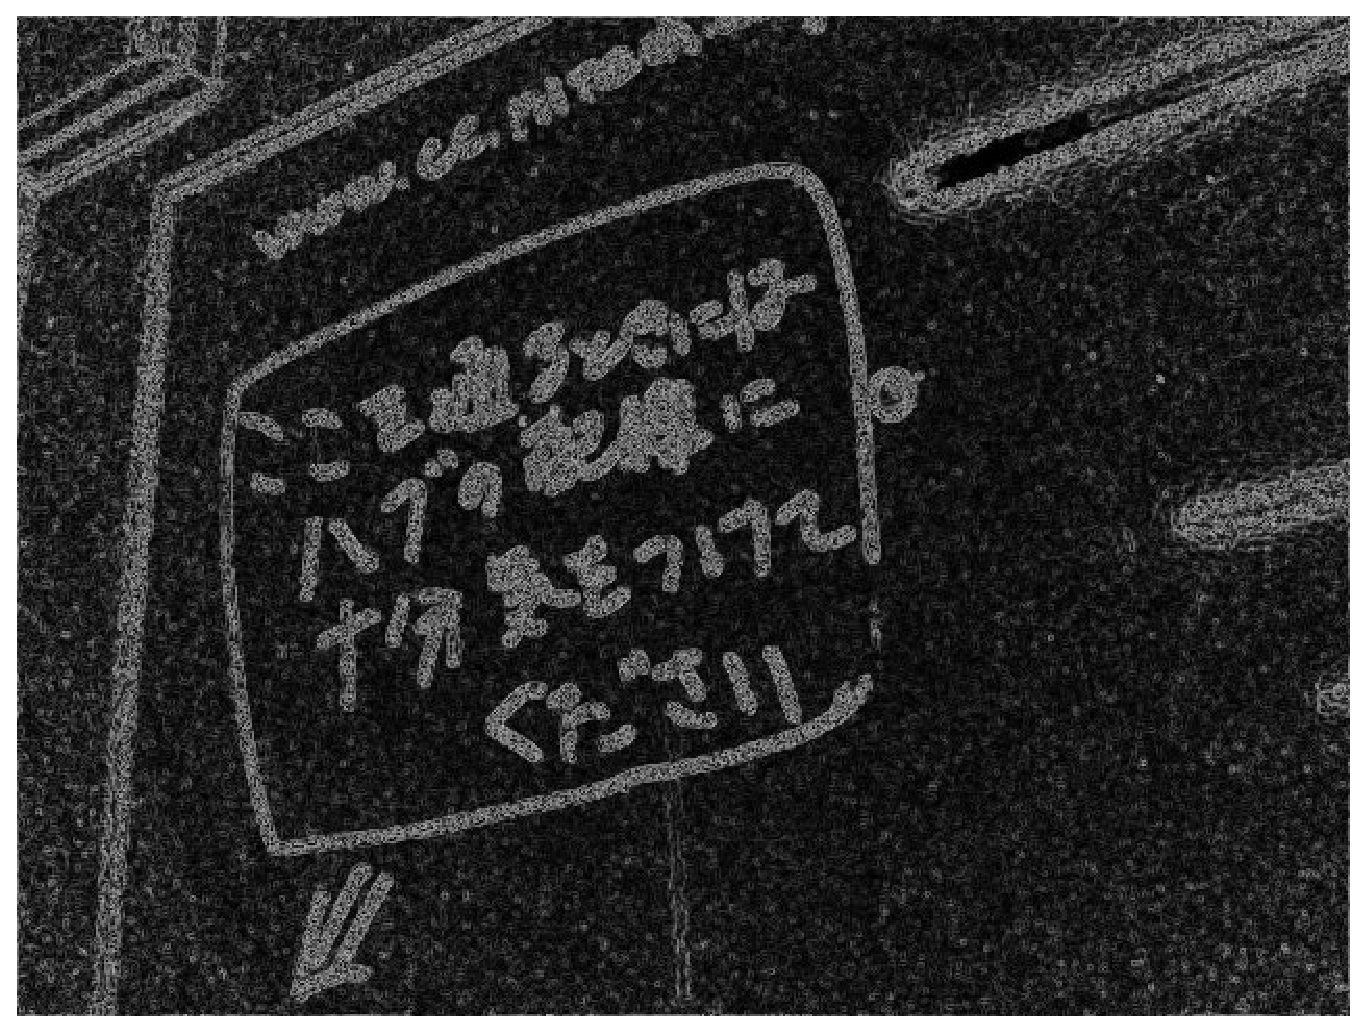
\includegraphics[width=\hsize]{./eps/edge-sobelin.eps}
   %% 分割されたサイズぴったりに図を掲載(width=\hsize)
   図14:Sobelフィルタによる実装
 \end{minipage}
 \begin{minipage}{0.49\hsize} % 横幅 x 0.49 のサイズで分割
   \center
   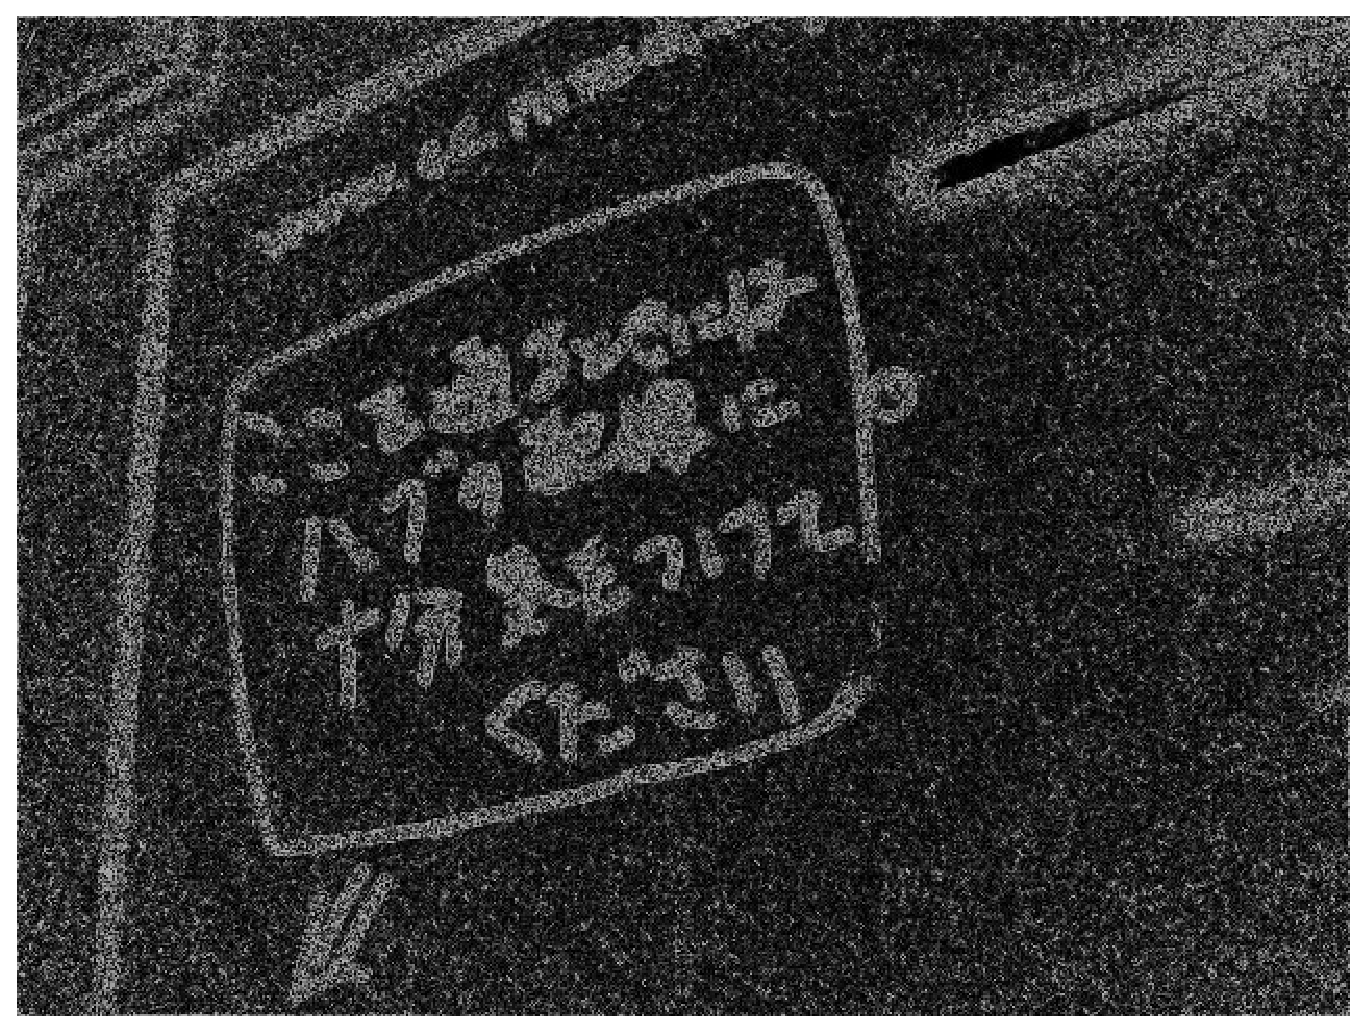
\includegraphics[width=\hsize]{./eps/edge-lapcianin.eps}

   %% 分割されたサイズぴったりに図を掲載(width=\hsize)
  図15:ラプラシアンフィルタによる実装
 \end{minipage}
 %\caption{minipageの使用例}
 \label{fig:affine2}
\end{figure}
\subsubsection{そのフィルタの特性等について考察せよ。}
ラプラシアンフィルタは以下の通りである。
$$
\begin{pmatrix}
   -1 & -1 & -1 \\
   -1 &  8 & -1 \\
   -1 & -1 & -1 
\end{pmatrix}
$$
Sobelフィルタに比べてかなりノイズが多いことが読み取れる。これはラプラシアンフィルタの構造からして、注目している画素
の色を極度に強調させる特徴を持っているためであると考える。
つまり、画像に小さなノイズが乗っていたときにそのノイズを顕著に検出してしまうと考える。\\
しかしSobelフィルタよりも一つのフィルタで済み、実装が簡単という点が挙げられる。
計算量においては、ラプラシアンフィルタの方が少ないが、オーダーで考えると変わらない。したがって
Sobelフィルタの方が、実装を少し頑張れば実用性があると考える。
%\subsubsection{知見と考察}

\subsection{演習4:コントラスト補正による処理}

\subsubsection{線形濃度変換および非線型濃度変換のプログラムを作成し、コントラストを補正せよ。}
\clearpage
\begin{figure}[tb]

 \begin{minipage}{0.49\hsize} % 横幅 x 0.49 のサイズで分割
   \center
   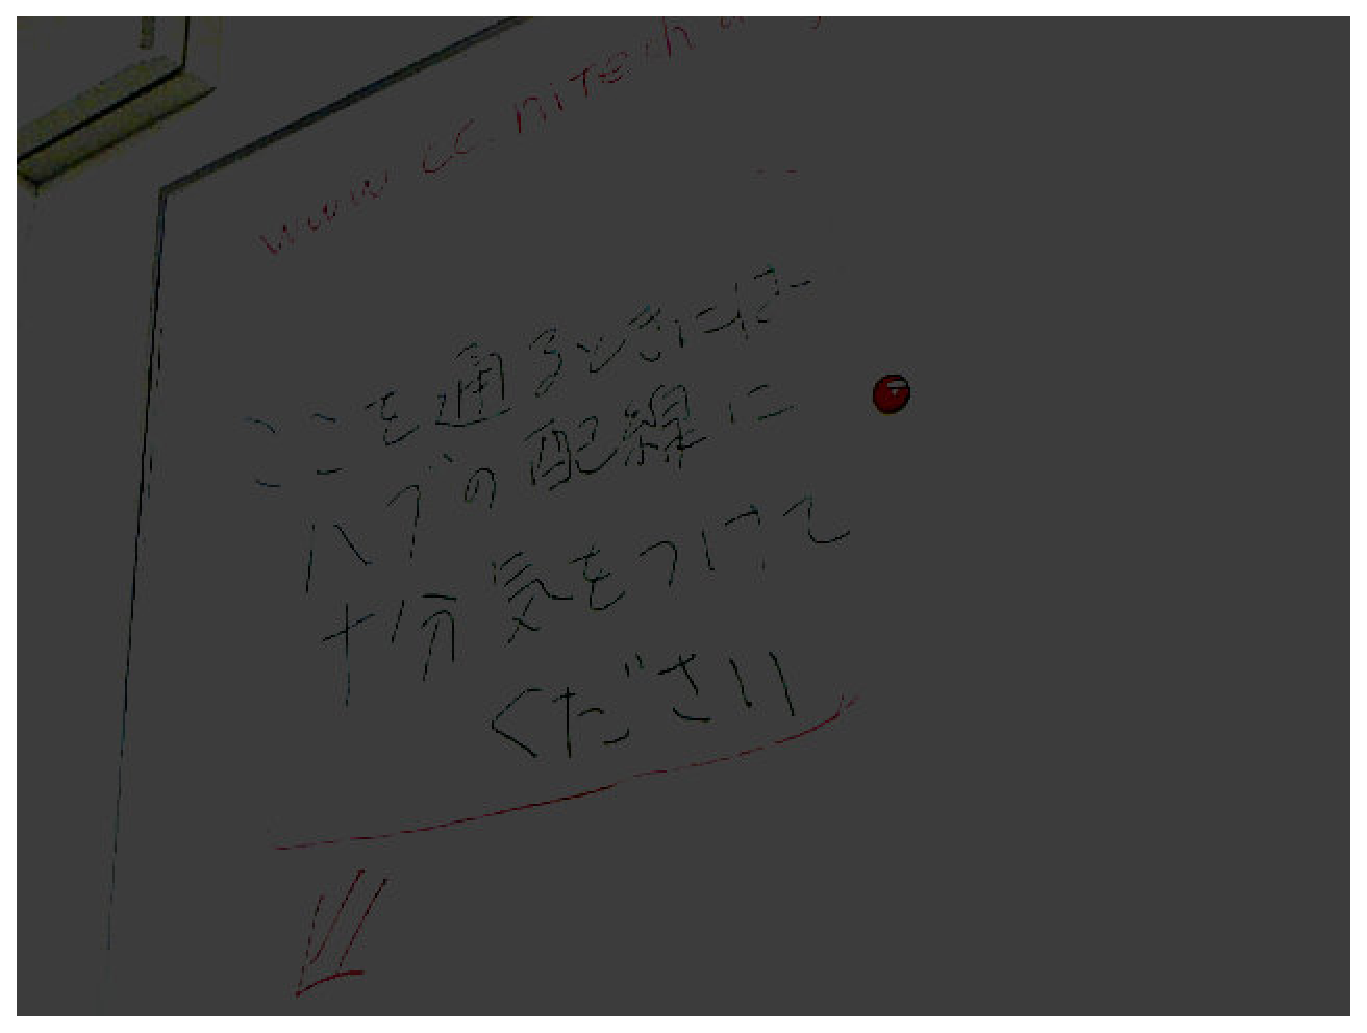
\includegraphics[width=\hsize]{./eps/contrast-linear-lowlow.eps}
   %% 分割されたサイズぴったりに図を掲載(width=\hsize)
   \\a=10,b=50,zm=60
 \end{minipage}
 \begin{minipage}{0.49\hsize} % 横幅 x 0.49 のサイズで分割
   \center
   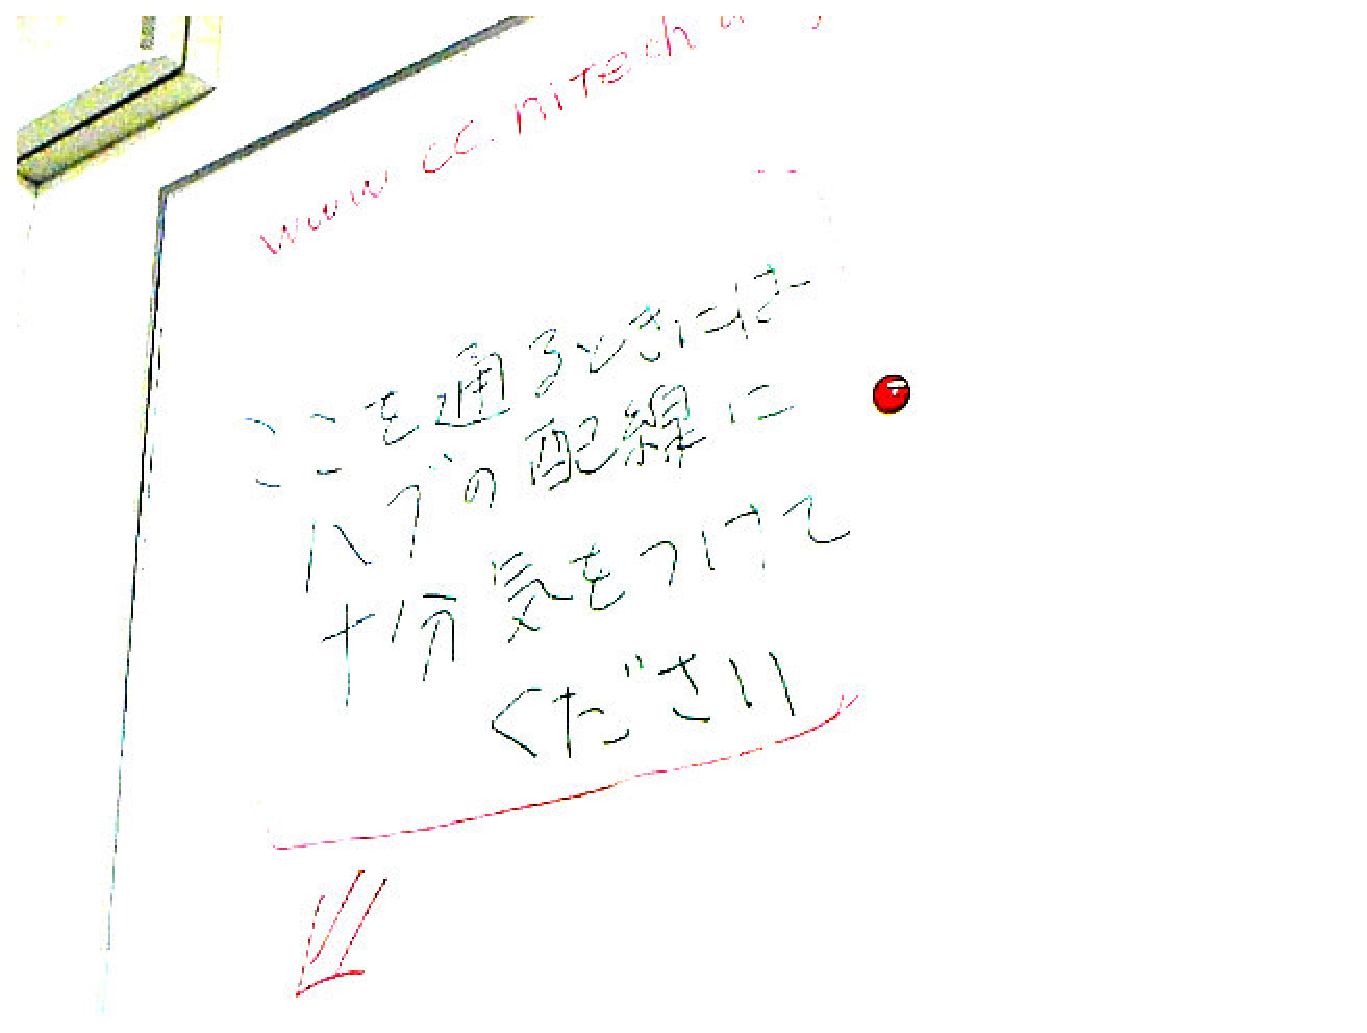
\includegraphics[width=\hsize]{./eps/contrast-linear-lowhigh.eps}
   %% 分割されたサイズぴったりに図を掲載(width=\hsize)
   \\a=10,b=50,zm=255
 \end{minipage}
 \begin{minipage}{0.49\hsize} % 横幅 x 0.49 のサイズで分割
   \center
   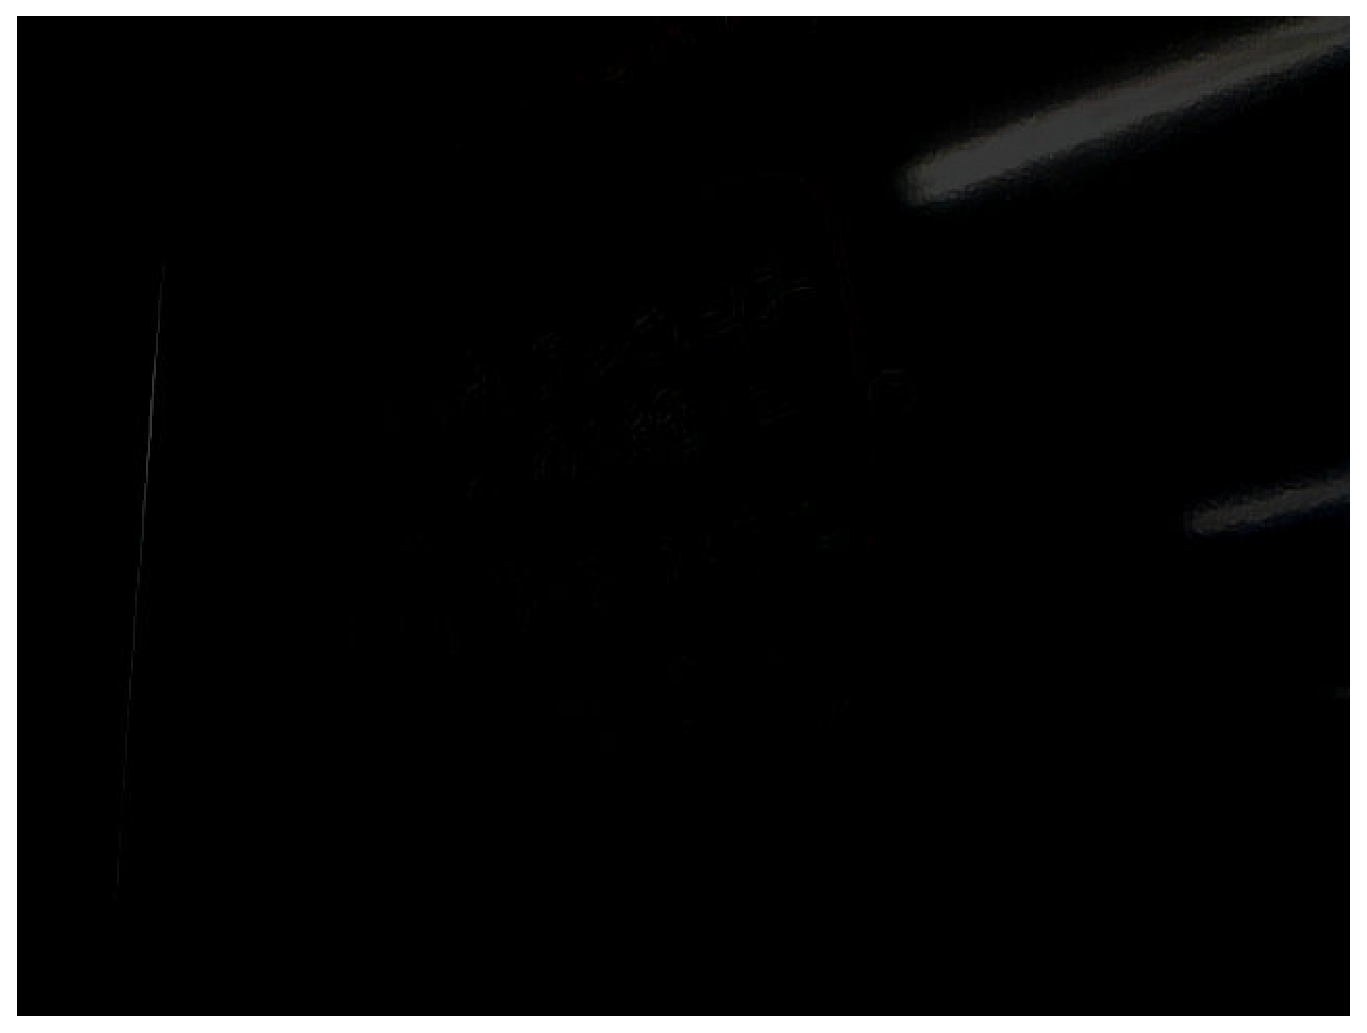
\includegraphics[width=\hsize]{./eps/contrast-linear-highlow.eps}
   %% 分割されたサイズぴったりに図を掲載(width=\hsize)
   \\a=150,b=250,zm=60
 \end{minipage}
 \begin{minipage}{0.49\hsize} % 横幅 x 0.49 のサイズで分割
   \center
   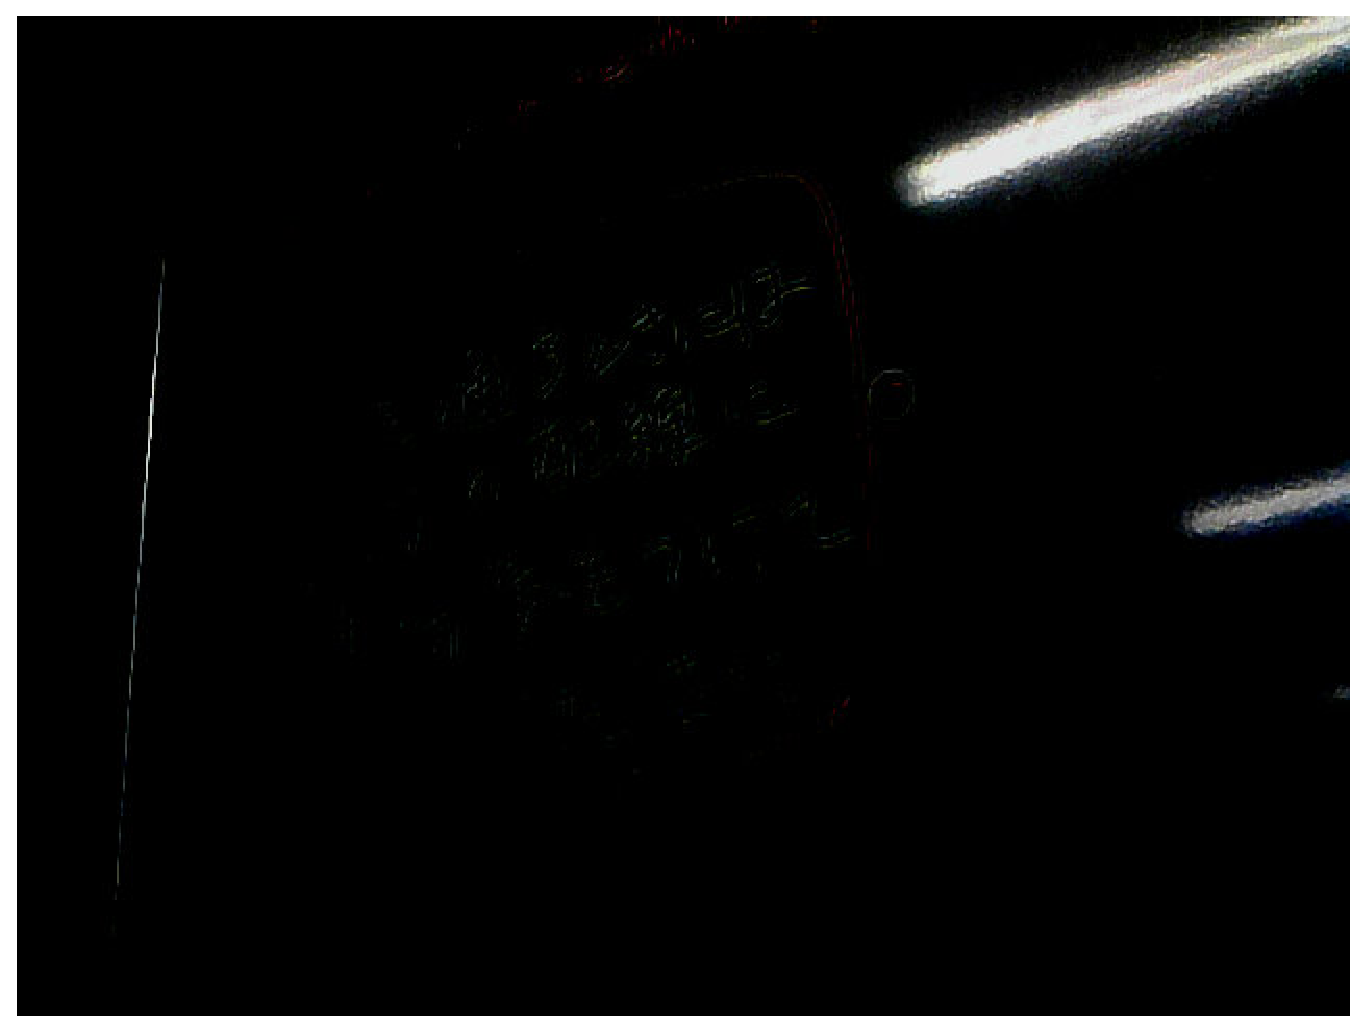
\includegraphics[width=\hsize]{./eps/contrast-linear-highhigh.eps}

   %% 分割されたサイズぴったりに図を掲載(width=\hsize)
   a=150,b=250,zm=225
 \end{minipage}
 \\
 図16:線形濃度変換
 \label{fig:affine2}
\end{figure}
\clearpage
\begin{figure}[tb]

 \begin{minipage}{0.49\hsize} % 横幅 x 0.49 のサイズで分割
   \center
   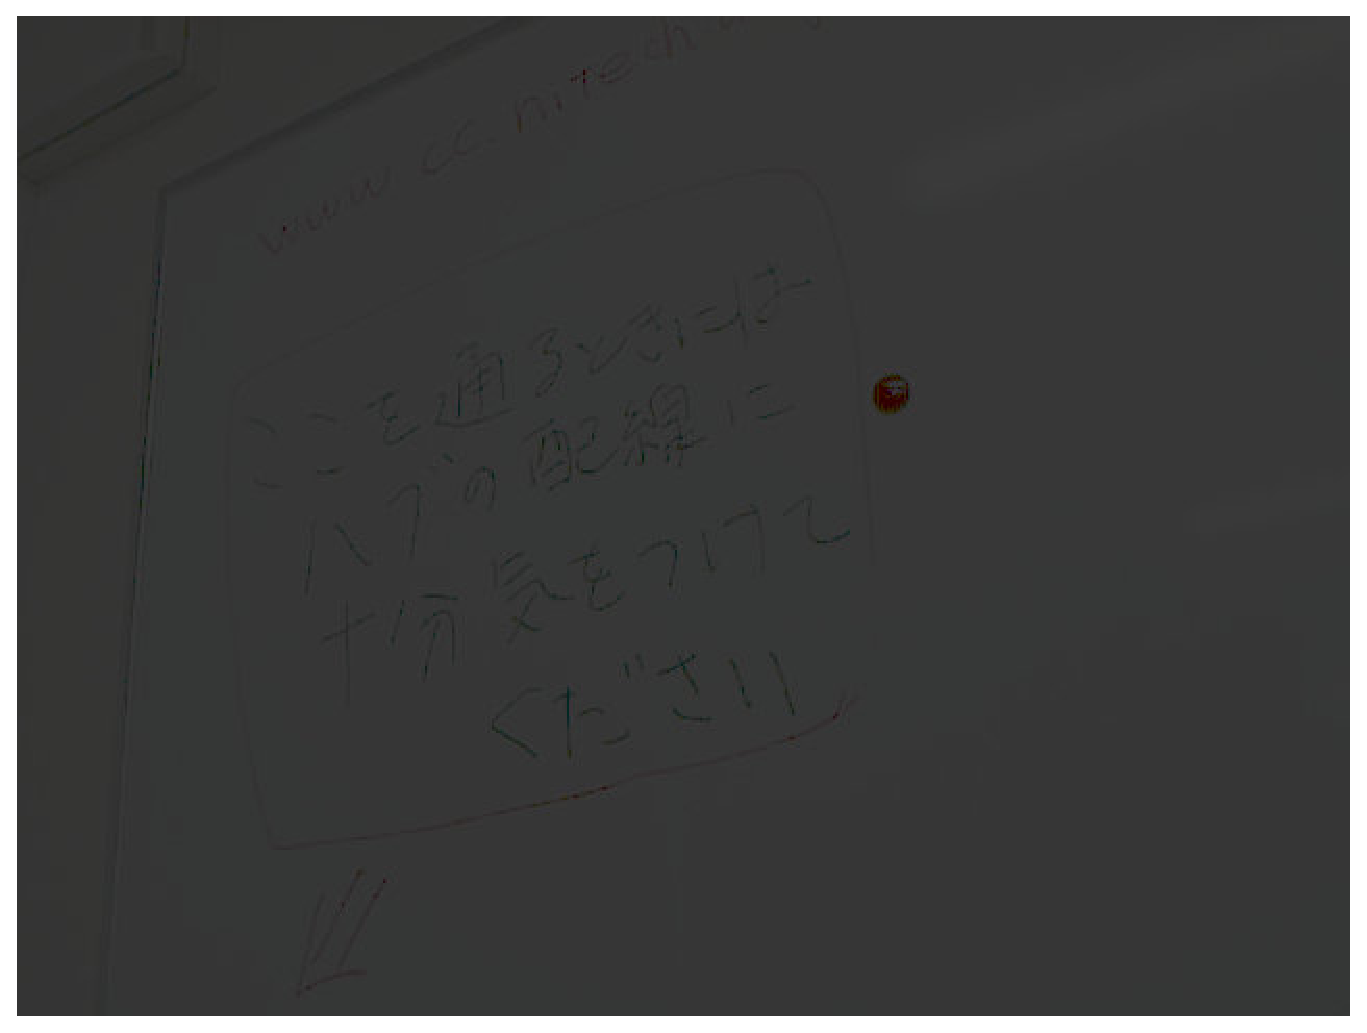
\includegraphics[width=\hsize]{./eps/contrast-notlinear-lowlow.eps}
   %% 分割されたサイズぴったりに図を掲載(width=\hsize)
  $\gamma=0.1$,zm=50
 \end{minipage}
 \begin{minipage}{0.49\hsize} % 横幅 x 0.49 のサイズで分割
   \center
%   \includegraphics[width=\hsize]{./eps/contrast-notlinear-lowhigh.eps}oooooooooooooooooooo
   %% 分割されたサイズぴったりに図を掲載(width=\hsize)
   %$$\gamma=0.1$$,zm=255
 \end{minipage}
 \begin{minipage}{0.49\hsize} % 横幅 x 0.49 のサイズで分割
   \center
   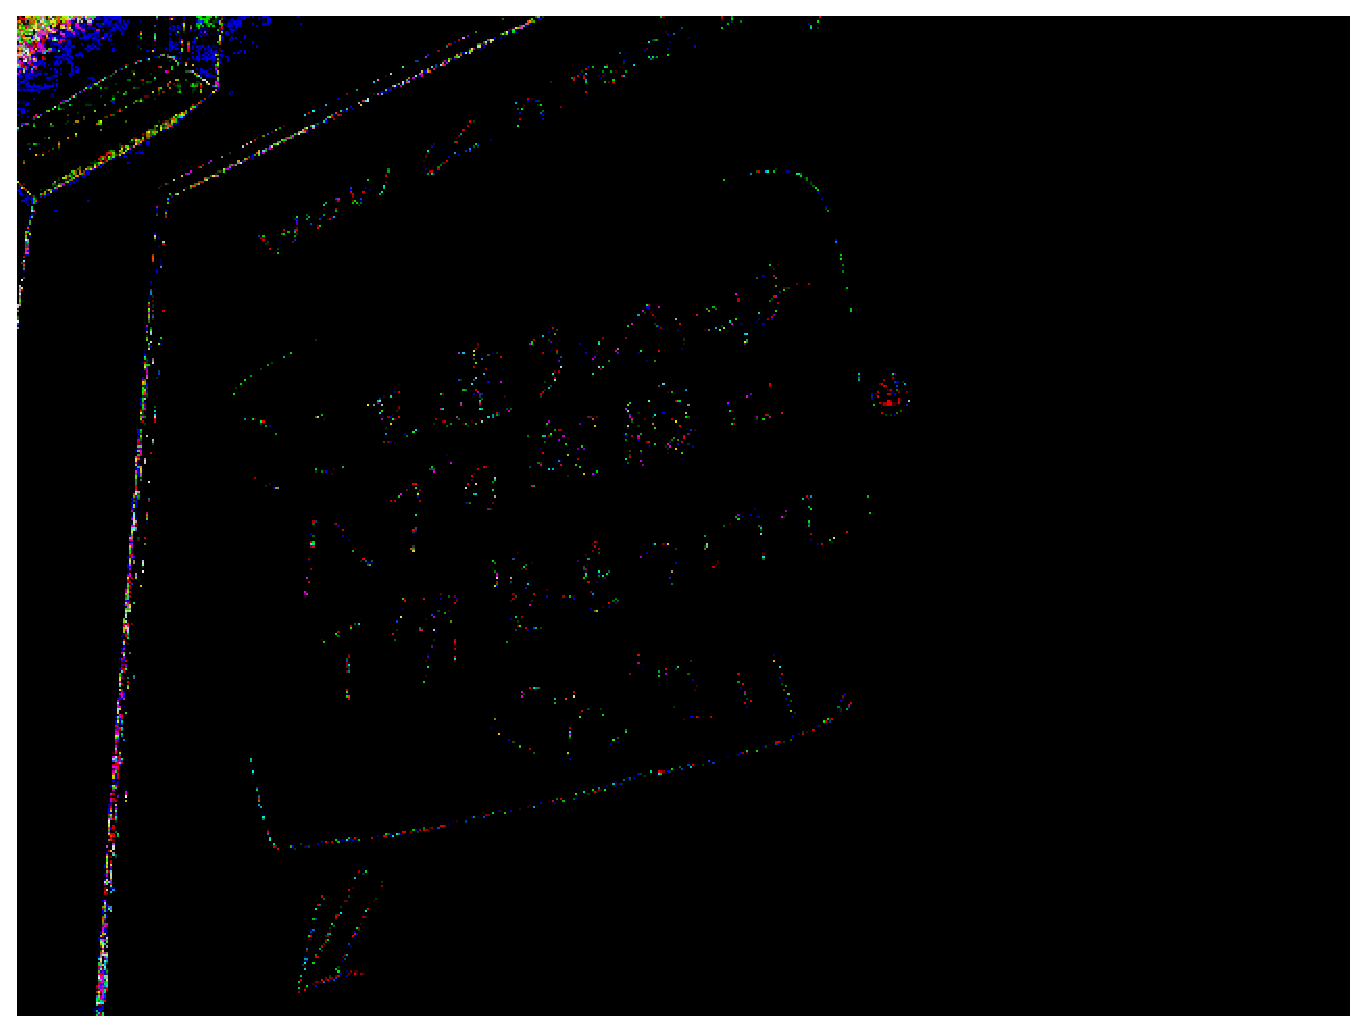
\includegraphics[width=\hsize]{./eps/contrast-notlinear-highlow.eps}
   %% 分割されたサイズぴったりに図を掲載(width=\hsize)
   $\gamma=100$,zm=50
 \end{minipage}
 \begin{minipage}{0.49\hsize} % 横幅 x 0.49 のサイズで分割
   \center
   
\includegraphics[width=\hsize]{./eps/contrast-notlinear-highhigh.eps}

   %% 分割されたサイズぴったりに図を掲載(width=\hsize)
   $\gamma=100$,zm=255
 \end{minipage}
 \\図17:非線形濃度変換
 \label{fig:affine2}
\end{figure}
\subsubsection{線形濃度変換の閾値や非線型濃度変換のガンマ値を変化させ、出力結果に与える影響を考察せよ}
考察は次セクションの知見と考察で示す。
\subsubsection{知見と考察}
線形濃度変換について、a,bをともに小さい値としたとき、かなり黒い画素のみ黒く残り、それ以外の画素はzmが大きければかなり明るく、
小さければ少し暗くなることが読み取れる。またa,bをともに大きい値にしたとき、かなり白い画素のみ白く残り、その画素はzmが大きければ
顕著に明るくなり、小さければ、少し暗くなり、またそれ以外の画素では真っ黒になることが読み取れる。よって、コントラストを上げるには
a,bの幅を小さく保ちながら適切な値に調節し、zmの値を大きくすることがよいと考える。またコントラストを下げるときは、a,bの幅を広くし、
zmの大きさを小さくすることがよいことがわかる。\\
非線型濃度変換について、ガンマ値を1より小さくすると、画像全体が比較的明るくなり、逆に1より小さくすると比較的暗くなる。これは線形変換のグラフからもわかることである。
また、zmの値を大きくすると、コントラストが上がり、逆に小さくするとコントラストが下がることがわかる。
\subsection{演習5:二値化処理}

\subsubsection{二値化処理を行うプログラムを実装し、入力画像を二値化処理せよ。}
\clearpage
\begin{figure}[tb]

 \center
 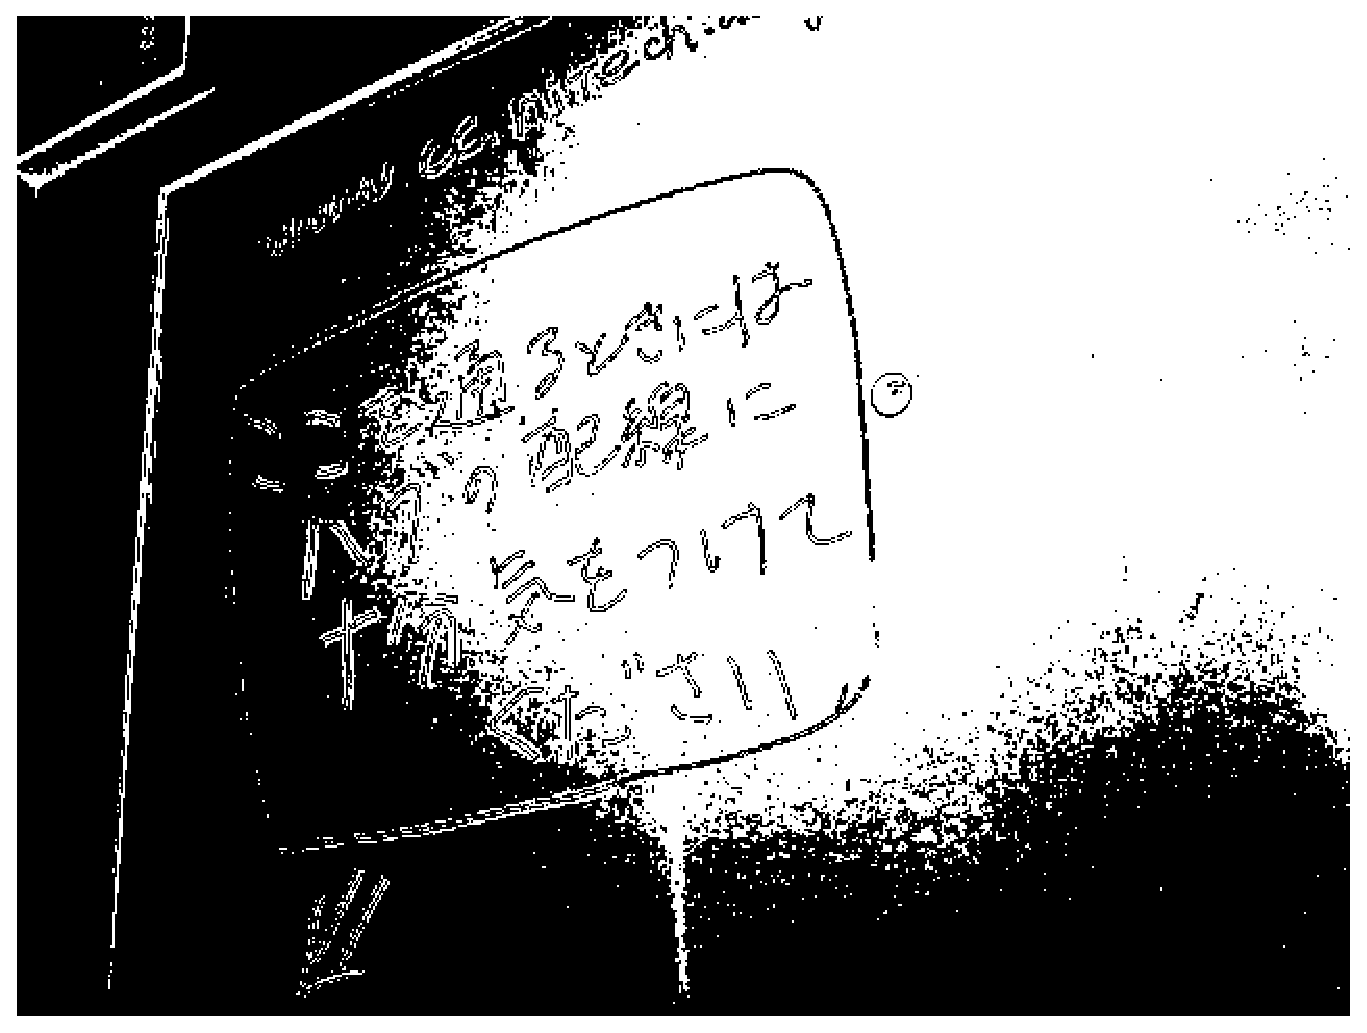
\includegraphics[width=0.8\hsize]{./eps/binarize-00.eps}
 %% 横幅 x 0.8 のサイズで図を掲載
   %% 最近はPDFファイルの使用が推奨されている(容量についても減少させやすい)
 \\図18:二値化画像
 \label{fig:affine1}

 \label{fig:affine2}
\end{figure}
\subsubsection{知見と考察}
人間の目によるRGBの明るさの割合を考慮して、R$\times$0.298+G$\times$0.586+B$\times$0.114の値が閾値より大きいか比べることによって出力した。
これをすることにより、人間の感覚にあった二値化処理が可能になる。\\
処理後の画像をみると、ホワイトボードの実際の色は一面真っ白であるにも関わらず、左下が黒で
右上が白くなっていて色がわかれている。これは、
画像の左半分は影により黒くなっており、右半分は蛍光灯の光が反射していて明るくなっているため、一つの画像に異なる明るさが
移り込んでいることが原因である。したがって、明るい場所と暗い場所がいっしょに映っている画像に関しては
二値化できる限度があると考える。\\
しかし、適切な二値化が行えれば、注目する領域を抽出できたり、RGBではデータ量を3分の1にすることができる。
\subsection{演習6:色による領域検出}

\subsubsection{色による領域検出処理を行うプログラムを実装せよ。}
\subsubsection{各自の顔画像を入力画像として使用し、顔を検出するように閾値を設定せよ。}
次セクションで示す。
\subsubsection{入力画像および出力画像、その際に用いた閾値を示し、処理結果について考察せよ。}
\clearpage
\begin{figure}[tb]

 \begin{minipage}{0.49\hsize} % 横幅 x 0.49 のサイズで分割
   \center
   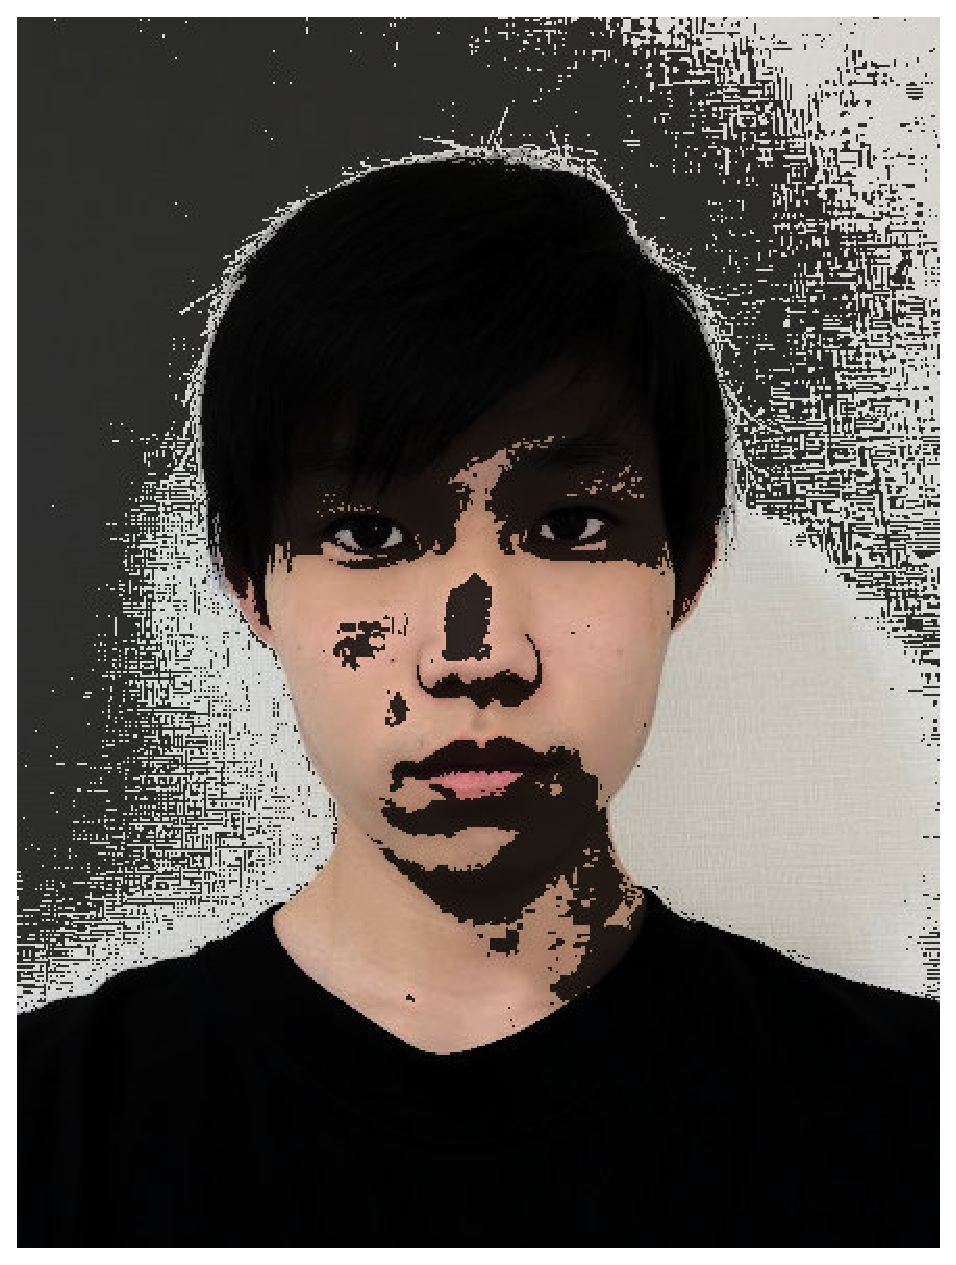
\includegraphics[width=\hsize]{./eps/color-myface.eps}
   %% 分割されたサイズぴったりに図を掲載(width=\hsize)
   図19:顔の領域検出
 \end{minipage}
 \begin{minipage}{0.49\hsize} % 横幅 x 0.49 のサイズで分割
   \center
   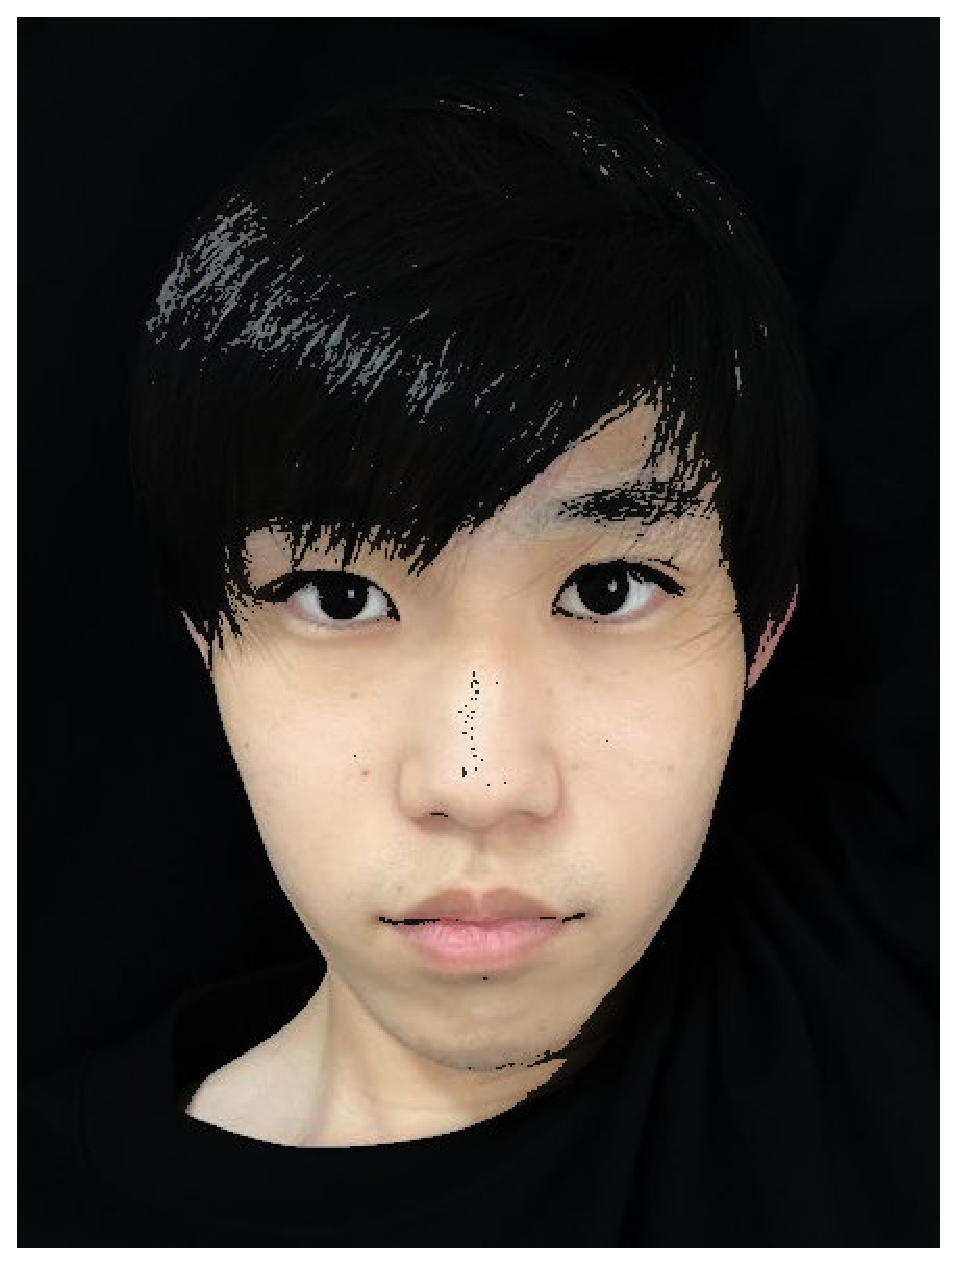
\includegraphics[width=\hsize]{./eps/color-myface2.eps}
   %% 分割されたサイズぴったりに図を掲載(width=\hsize)
   図20:背景の色をコートで隠した顔の領域検出
 \end{minipage}
 \
 %図16:線形濃度変換
 %\label{fig:affine2}
\end{figure}

考察は次セクションの知見と考察で示す。
\subsubsection{知見と考察}
顔の肌を検出することができたが、背景も同じような色であったため背景も検出されてしまった。そこで背景を紺色のコートで覆い、
改めて処理をしたら、顔の肌のみ検出することができた。\\
ほかの画像において、検出したいものの色と同じ色の物体や背景があることは多々あるので、注目したいものの領域のみを検出する場合には、
何か違う処理と組み合わせて実装する必要があると考えた。


%\subsection{応用課題3:コントラスト補正による処理}

%\subsubsection{画像のヒストグラムについて調査し、ヒストグラムを表示するプログラムを実装せよ。}
%\subsubsection{任意の画像についてのコントラスト補正前後のヒストグラムを作成し、コントラスト補正についてヒストグラムの観点からについて考察せよ。}

%\subsubsection{知見と考察}

\subsection{演習7:背景差分処理}

\subsubsection{背景差分処理を行うプログラムを実装せよ。}
\subsubsection{カメラを固定し、背景画像を撮影し、オブジェクトを全面に表示し、背景画像との差分をとることにより、物体を検出せよ。}
\clearpage
\begin{figure}[tb]

\center
 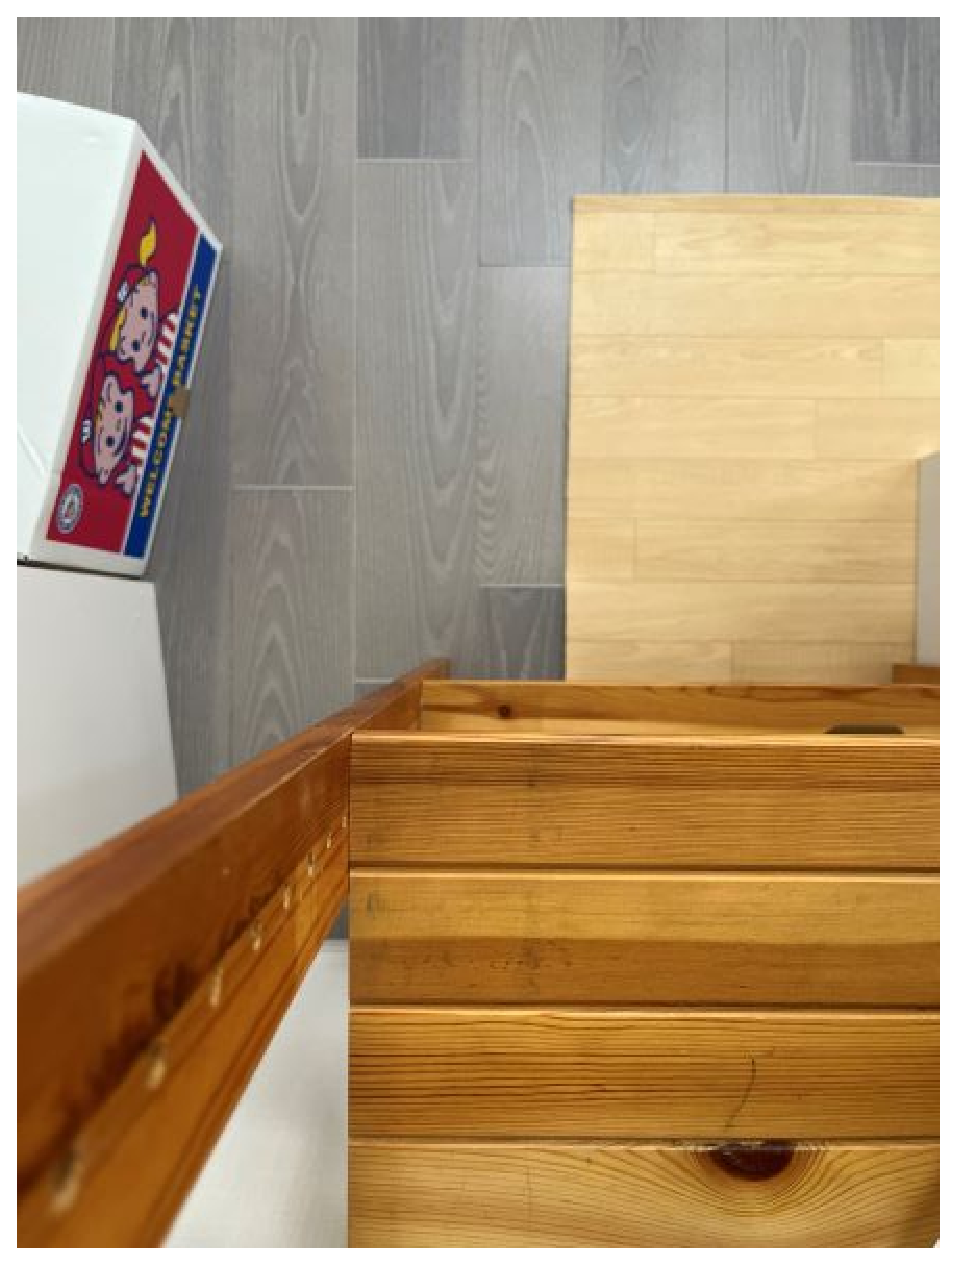
\includegraphics[width=0.7\hsize]{./eps/no_exist.eps}
 %% 横幅 x 0.8 のサイズで図を掲載
   %% 最近はPDFファイルの使用が推奨されている(容量についても減少させやすい)
 \\図21:背景画像
 \label{fig:affine1}
 \clearpage
 \begin{minipage}{0.49\hsize} % 横幅 x 0.49 のサイズで分割
   \center
   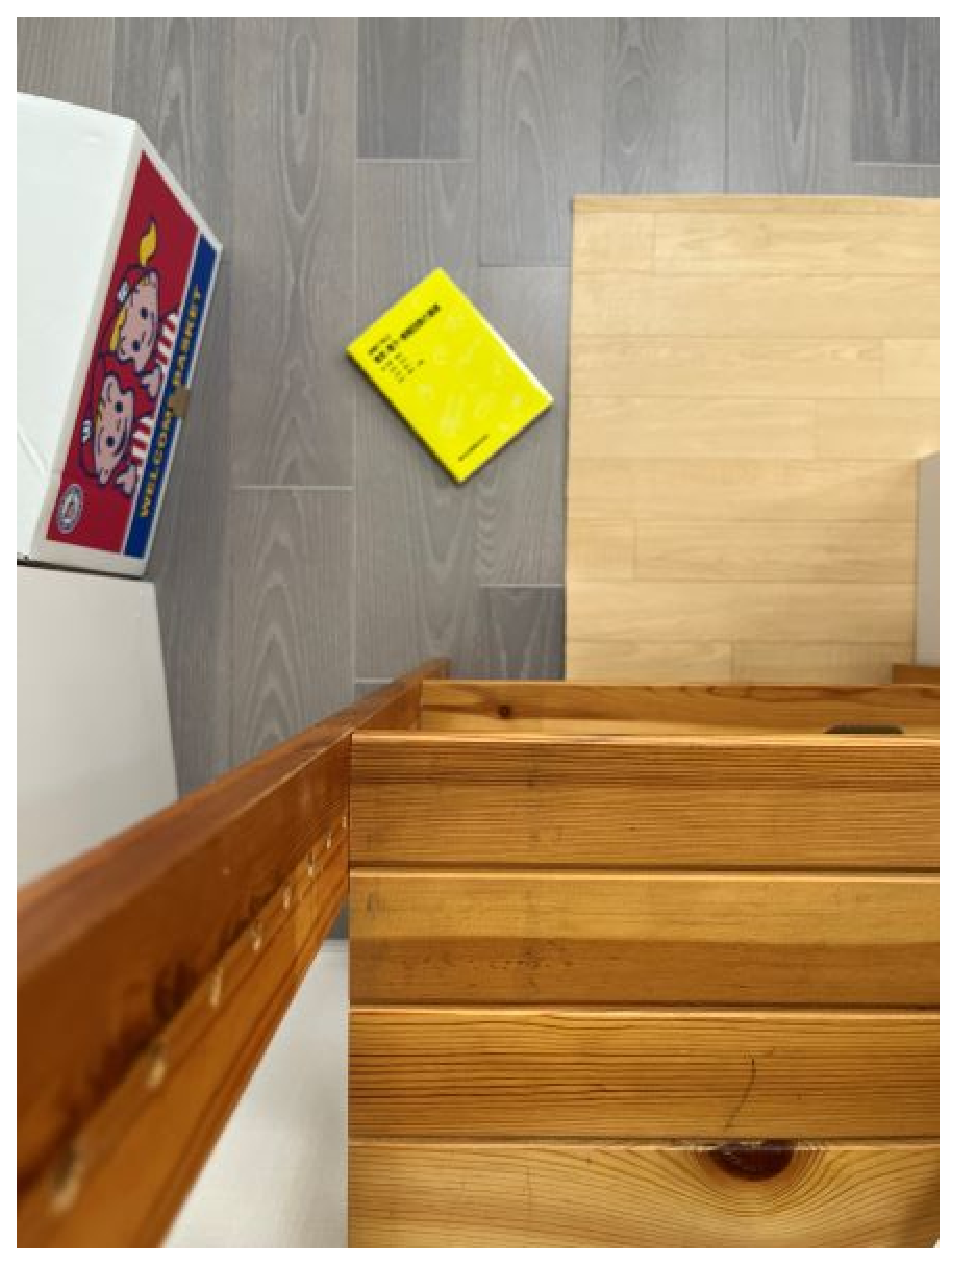
\includegraphics[width=0.7\hsize]{./eps/exist.eps}
   %% 分割されたサイズぴったりに図を掲載(width=\hsize)
   \\図22:物体のある画像
 \end{minipage}
 \begin{minipage}{0.49\hsize} % 横幅 x 0.49 のサイズで分割
   \center
   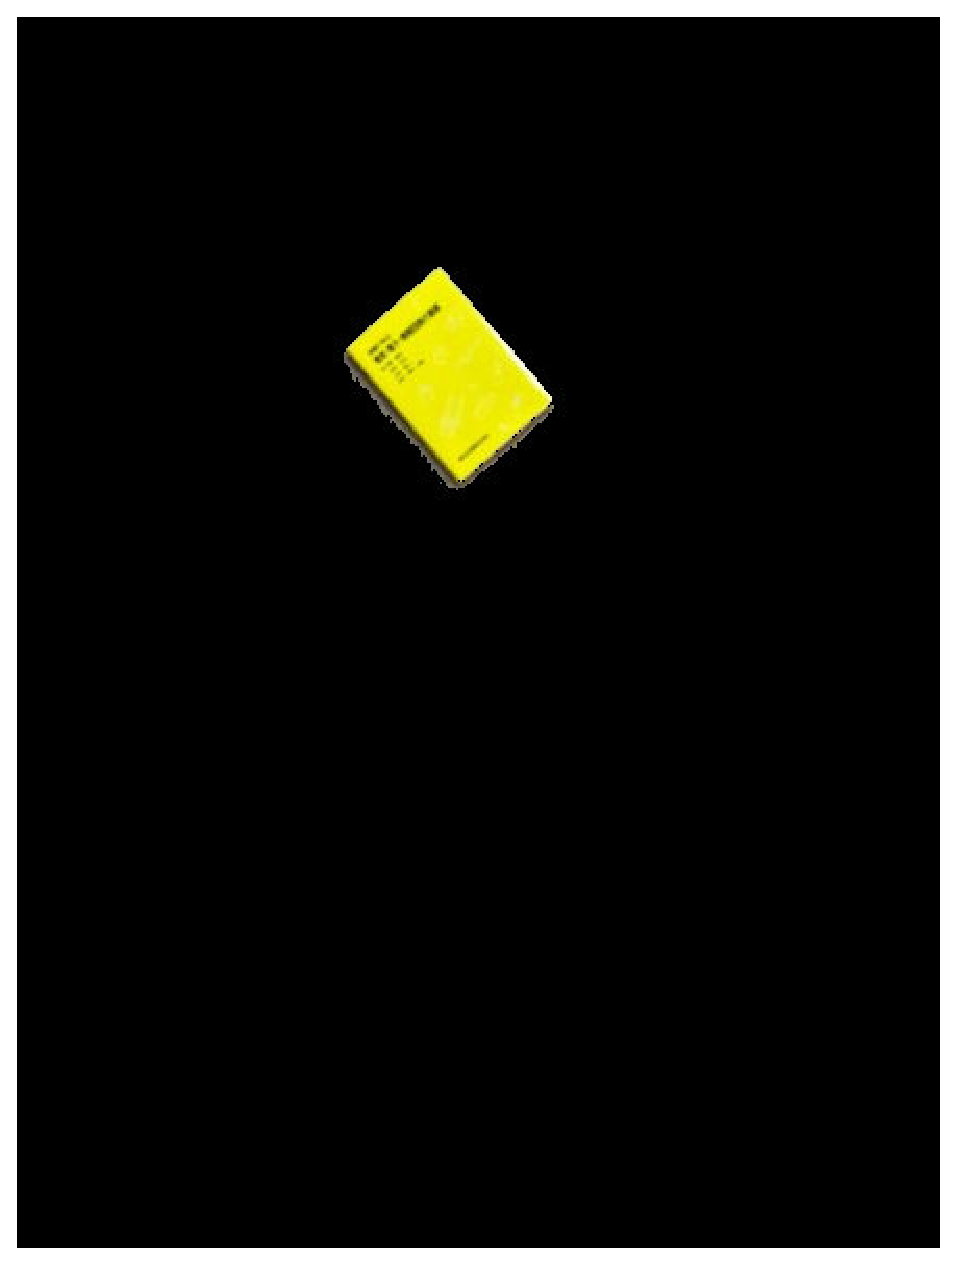
\includegraphics[width=0.7\hsize]{./eps/back-electric.eps}
   %% 分割されたサイズぴったりに図を掲載(width=\hsize)
   \\図23:検出結果画像
 \end{minipage}
 \
 %\caption{図16:線形濃度変換}
 \label{fig:affine2}
\end{figure}
\subsubsection{知見と考察}
うまく指導書が検出できている。しかし、これは指導書が床の色と似ていなかったためであり、仮に似ていたとしたら検出にノイズが入ってしまうと考える。
また、背景との差分をとっていて、カメラを固定することが前提となってしまっている。
しかし、検出の精度は演習6の色による領域検出処理よりは上がっており、物体のなかったところを誤って検知してしまったりすることがないので
たとえば監視カメラなど、カメラを固定できるという条件をのむことができれば、十分に有用性があると考えた。
\subsection{演習8:フレーム間差分処理}
\clearpage
\begin{figure}[tb]



 \begin{minipage}{0.49\hsize} % 横幅 x 0.49 のサイズで分割
   \center
   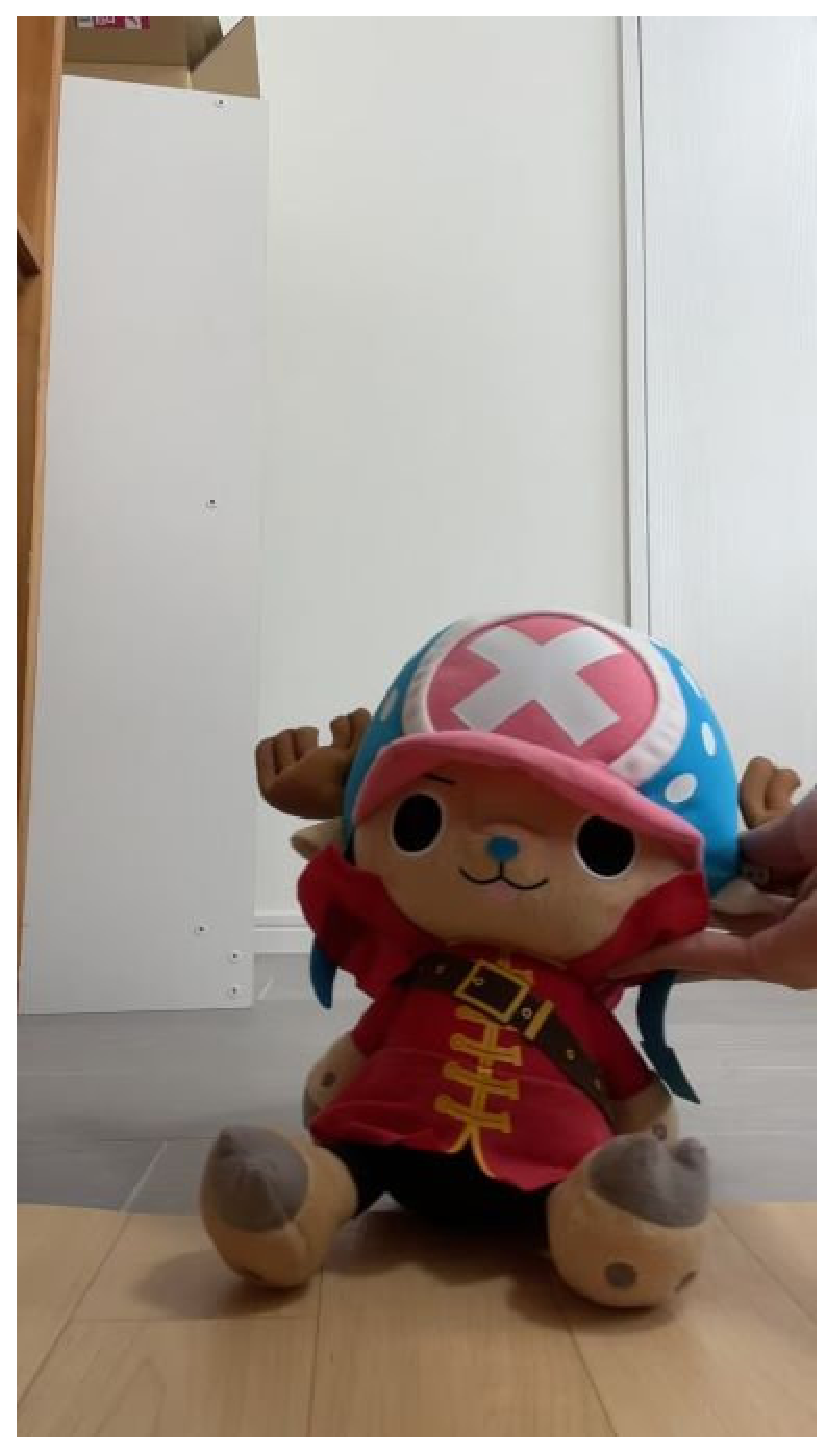
\includegraphics[width=0.6\hsize]{./eps/frame-thopper1.eps}
   %% 分割されたサイズぴったりに図を掲載(width=\hsize)
 \end{minipage}
 \begin{minipage}{0.49\hsize} % 横幅 x 0.49 のサイズで分割
   \center
   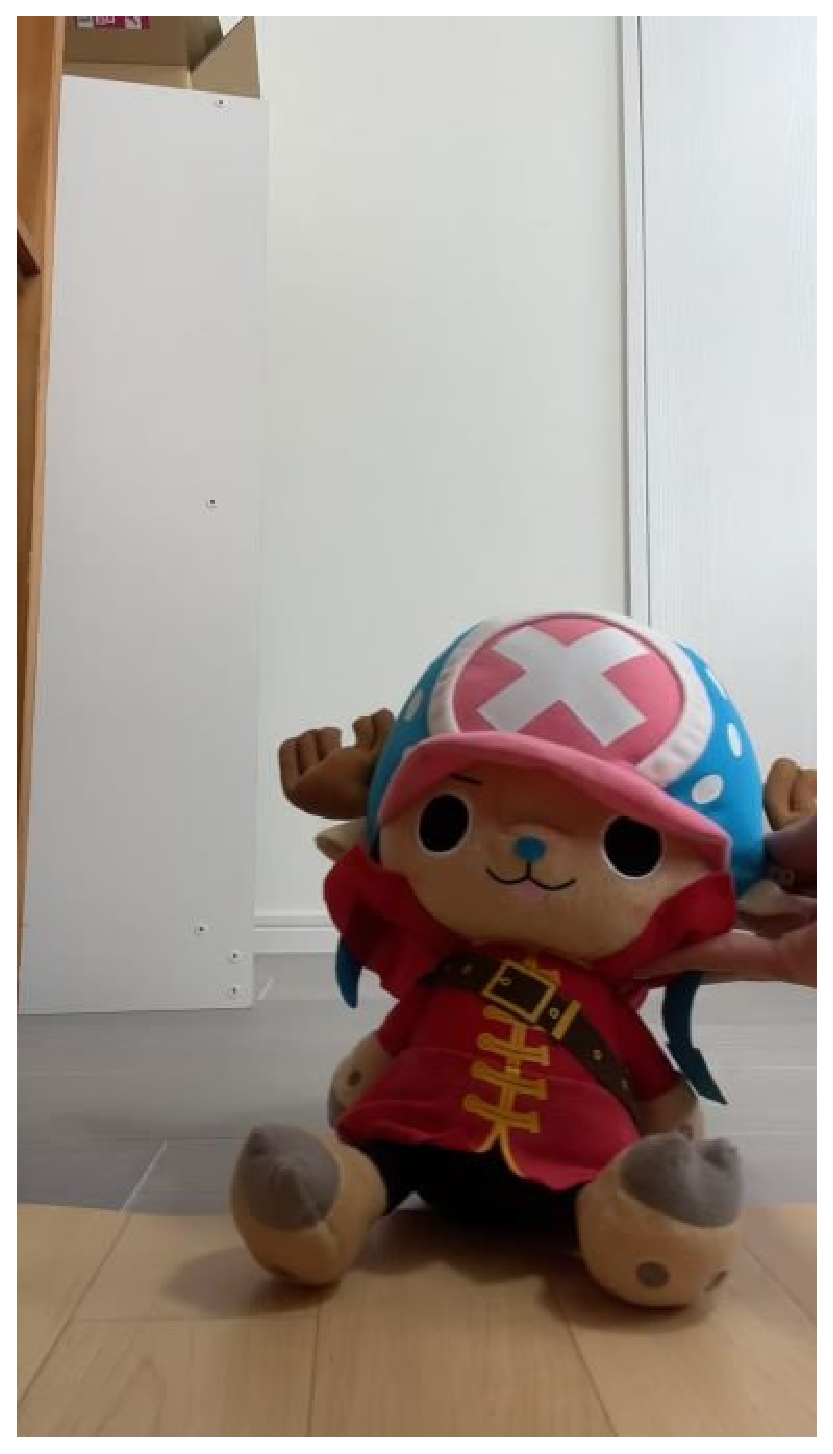
\includegraphics[width=0.6\hsize]{./eps/frame-thopper2.eps}
   %% 分割されたサイズぴったりに図を掲載(width=\hsize)
 \end{minipage}
 \
 \\図24:フレーム
 \label{fig:affine2}
 \clearpage
 \center
 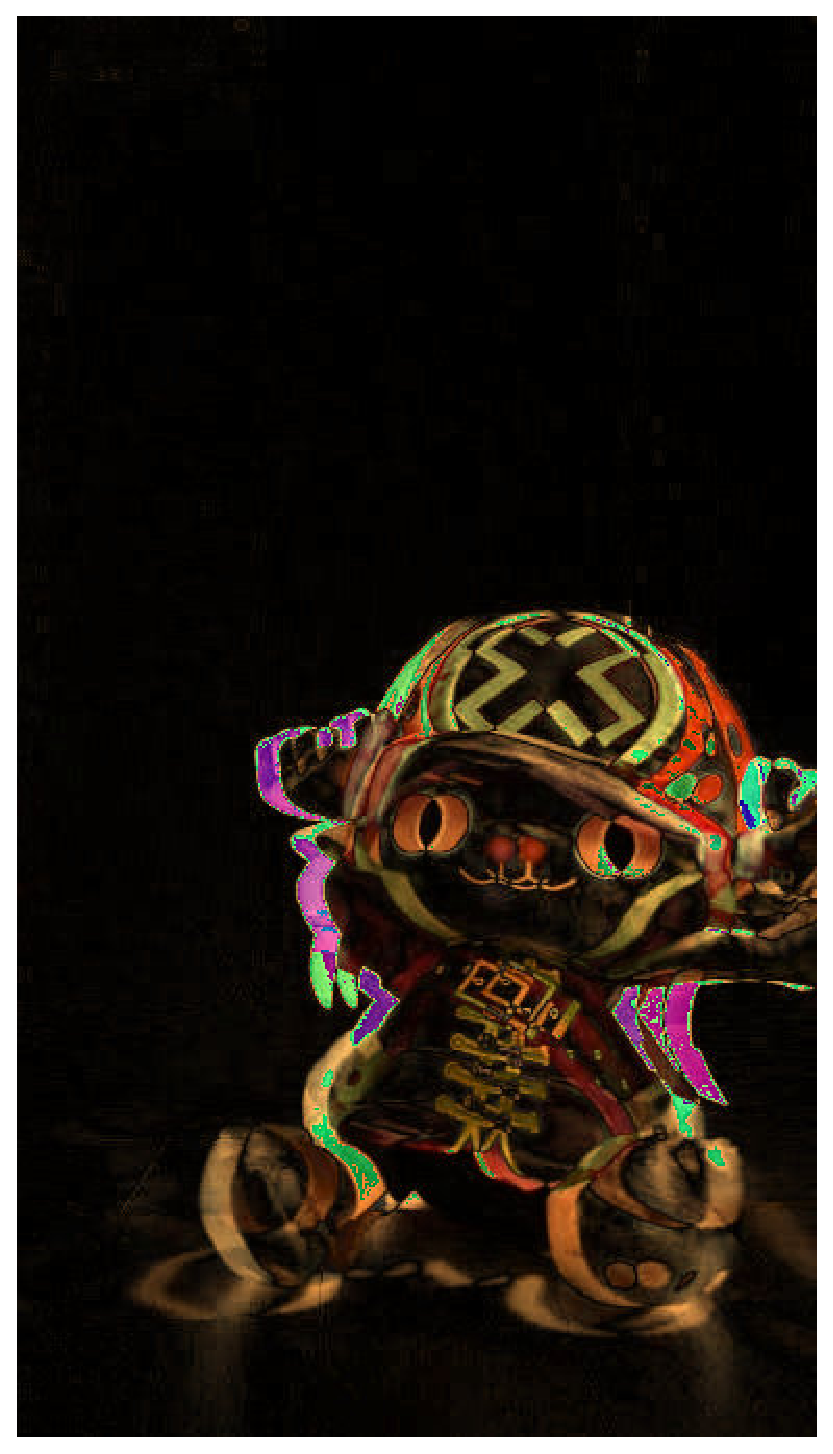
\includegraphics[width=0.5\hsize]{./eps/frame-thopper3.eps}
 %% 横幅 x 0.8 のサイズで図を掲載
   %% 最近はPDFファイルの使用が推奨されている(容量についても減少させやすい)
 \\図25:フレーム間差分処理結果
 \label{fig:affine1}
\end{figure}
\subsubsection{フレーム間差分処理を行うプログラムを実装せよ。}
\subsubsection{カメラを固定し、動画像を撮影し、物体を移動させ、フレーム監査文をとることにより、物体を検出せよ。}
\subsubsection{あるフレームの入力画像およびフレーム間差分画像を示し、処理結果について考察せよ。}
考察は次セクションの知見と考察で示す。
\subsubsection{知見と考察}
フレーム間差分を行うことによって画像の名かで動かしたキャラクターの輪郭が検出された。フレーム間差分処理は
、あらかじめ背景画像をとる必要がないという点で、背景画像の取得が困難な場合に有効であると考えた。しかし、
演習結果からわかる通り、色まで検出できないという欠点がある。
\subsection{演習9:テンプレートマッチングによる画像認識}

\subsubsection{テンプレートマッチングを行うプログラムを実装せよ。}
\subsubsection{入力画像に対してテンプレートマッチングを行い、テンプレート画像が検出されるか確認せよ。}
\subsubsection{次にフィルタ処理や二値化処理を組み合わせた場合の結果について考察せよ。}
\clearpage
\begin{figure}[tb]

 \begin{minipage}{0.49\hsize} % 横幅 x 0.49 のサイズで分割
   \center
   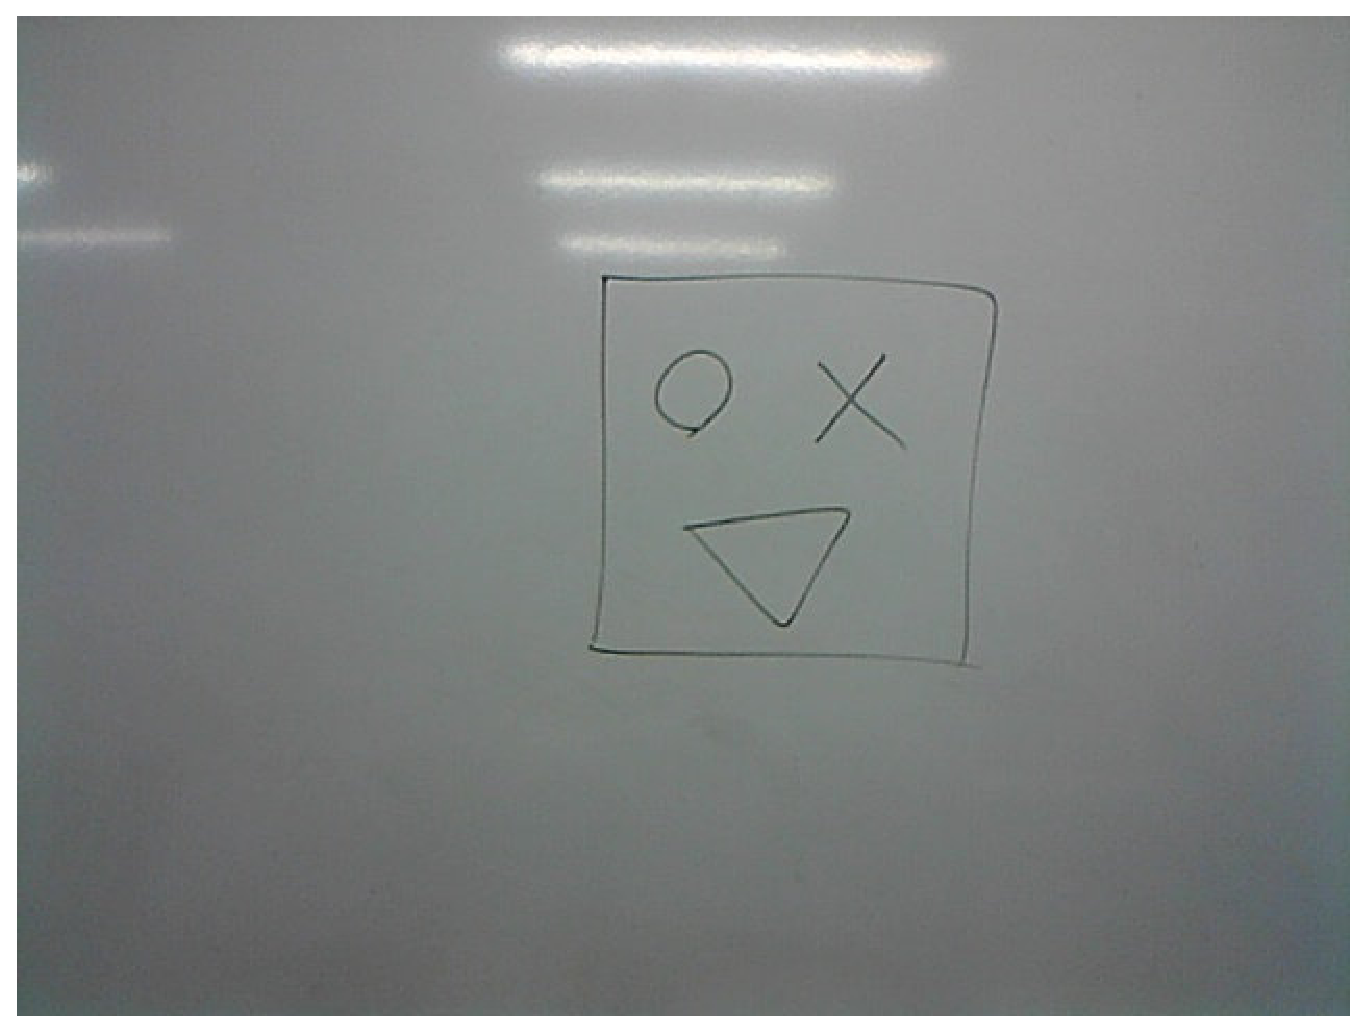
\includegraphics[width=\hsize]{./eps/template-04-in.eps}
   %% 分割されたサイズぴったりに図を掲載(width=\hsize)
   図26:未処理元画像
 \end{minipage}
 \begin{minipage}{0.49\hsize} % 横幅 x 0.49 のサイズで分割
   \center
   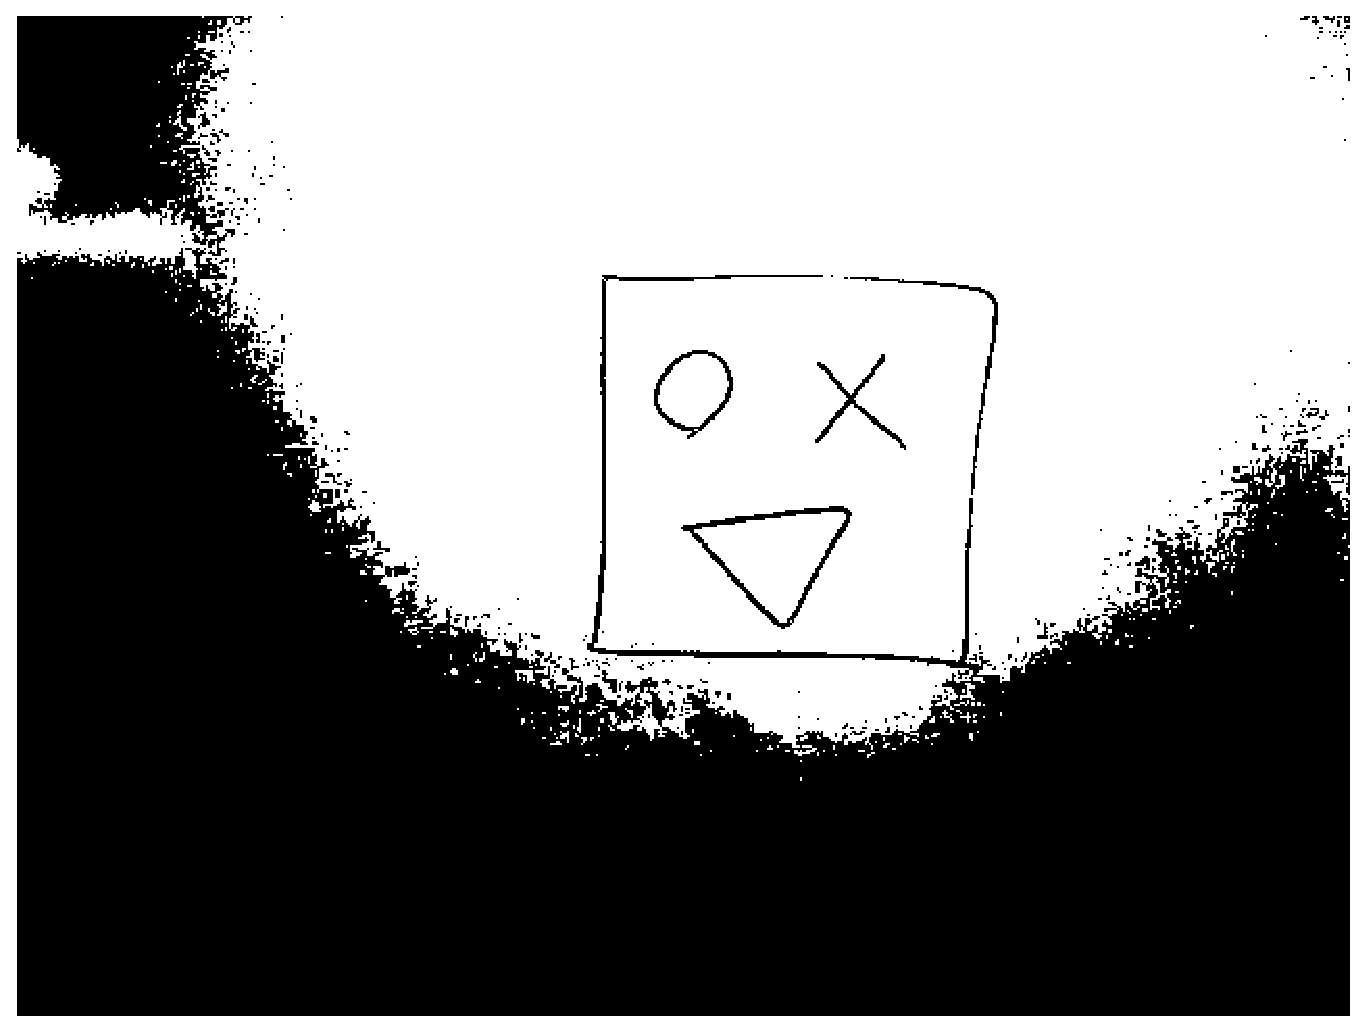
\includegraphics[width=\hsize]{./eps/template-00-in.eps}

   %% 分割されたサイズぴったりに図を掲載(width=\hsize)
  図27:二値化処理元画像
 \end{minipage}
 %\caption{minipageの使用例}
 \label{fig:affine2}
 \begin{minipage}{0.49\hsize} % 横幅 x 0.49 のサイズで分割
   \center
   
\includegraphics[width=\hsize]{./eps/template-04.eps}
   %% 分割されたサイズぴったりに図を掲載(width=\hsize)
   図28:テンプレートマッチング処理後
 \end{minipage}
 \begin{minipage}{0.49\hsize} % 横幅 x 0.49 のサイズで分割
   \center
   
\includegraphics[width=\hsize]{./eps/template.eps}

   %% 分割されたサイズぴったりに図を掲載(width=\hsize)
  図29:二値化処理後のテンプレートマッチング
 \end{minipage}

 \begin{minipage}{0.49\hsize} % 横幅 x 0.49 のサイズで分割
   \center
   
\includegraphics[width=\hsize]{./eps/template-04.eps}
   %% 分割されたサイズぴったりに図を掲載(width=\hsize)
   図30:テンプレート画像
 \end{minipage}
 \begin{minipage}{0.49\hsize} % 横幅 x 0.49 のサイズで分割
   \center
   
\includegraphics[width=\hsize]{./eps/binarytemplate.eps}

   %% 分割されたサイズぴったりに図を掲載(width=\hsize)
  図31:二値化処理のテンプレート画像
 \end{minipage}

\end{figure}
考察は次セクションの知見と考察で示す。
\subsubsection{知見と考察}
私の実装したテンプレートマッチングではfor文の入れ子が6重になったので、結果が出るまで約3分ほど時間がかかった。
今回はSADで行ったので、3分ほどで終わったが、NCCなどのさらに計算量の多い処理をすると実用性がなくなるので、もっと良いアルゴリズムを
取り入れる必要があると考えた。\\
原画像のままのテンプレートマッチングも二値化処理後のものも同じ場所を抜き出していることが読み取れる。
%

% 演習1〜9まで必ず記載すること.
% 実験結果から得られた知見や考察も必ず記入すること.
%
\section{まとめ}
%
%
1から9の演習を通して様々な画像処理の方法について学んだ。入力画像に影があったりなかったりすることに
左右されるフィルタがたくさんあり、影などの問題に対抗できるようなフィルタを用いれば世の生活に
行かせるのではないかと考えた。また、今回習った基本的な処理だけでも、組み合わせることでより複雑な画像処理が
できるので、今回学んだことは非常に重要であると考える。
%

%
%
\section{感想}
%
% 実験を行った感想や改善してほしいこと等,書いて下さい.
%
実際に動画像においてフレーム差分処理を行うとき、たとえば車の自動ブレーキシステムでは、入力されてから
出力されるまで一刻も速くしなければならないので、そのためのアルゴリズムはどうなっているのか気になった。\\
また、今回習ったフィルタ以外でも、さらに便利なフィルタがあると思ったので調べてみたいと思った。\\
今回の演習では、関数の定義だけ学んだが、そのほかの部分は先生がつくっているので、その部分が実際にどう動いているのか、
時間が空いたときに見たいと思った

%
%
\end{document}

